\section{Results: a 500\,nm Hexagonal Single Crystal to 10\,dpa}
\label{sec:results}

Every result below comes from one calculation: the calibrated parameter set of
\cref{tab:fitted}, all nine families, three moments each, peripheral emission
active, the basal chain inactive, and the grain-boundary loop channel of
\cref{sec:gb-loops} active. Conditions are $T=573\,$K,
$G=10^{-7}\,\mathrm{dpa\,s^{-1}}$, zero applied stress, and eight dose intervals
from $10^{-4}$ to 10\,dpa. Where a comparison is drawn against the same case
\emph{without} the loop channel, that companion differs in nothing else.

\subsection{Geometry, discretization and system size}
\label{sec:geometry}

The domain is a hexagonal prism of 500\,nm across flats and 800\,nm along
$[0001]$, meshed with a refined boundary layer 100\,nm deep in which the target
element size falls from 60 to 20\,nm (\cref{fig:mesh}). The refinement is not
cosmetic: \cref{sec:results-mobile} measures interstitial boundary layers of
$16$--$28\,$nm, so an unrefined mesh at $60\,$nm would resolve the steepest
gradient in the problem with a single element.

\begin{figure}[htbp]
\centering
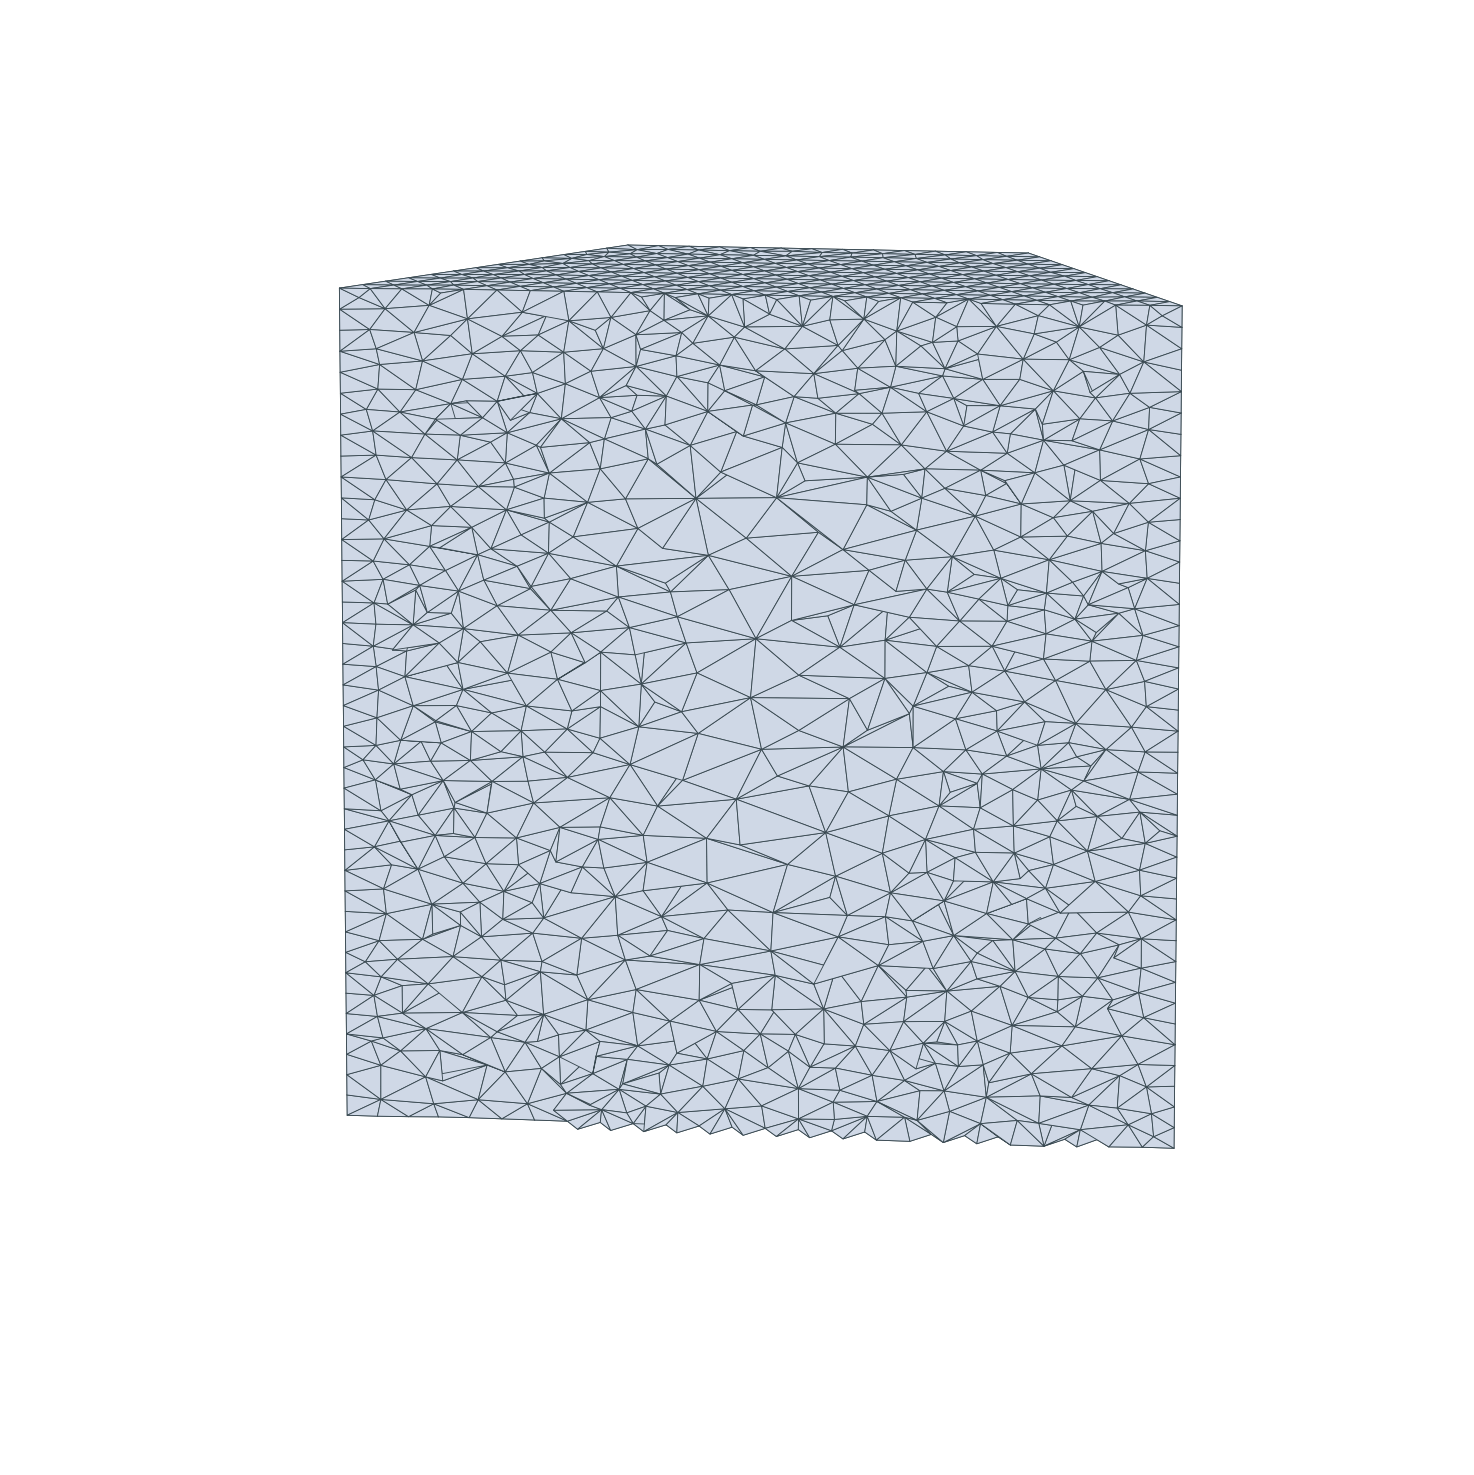
\includegraphics[width=0.55\textwidth]{figures/fe_mesh.png}
\caption{The finite-element mesh, cut in half so that the interior is visible:
60\,922 tetrahedra on 12\,581 mesh vertices. The refinement toward the six
prismatic faces and the two basal faces is the boundary layer, 100\,nm deep,
within which the element size falls from 60 to 20\,nm. Crystal axes as in
\cref{fig:hcp-cell}: $[10\bar10]$, $[\bar2\bar1\bar10]$ and $[0001]$.}
\label{fig:mesh}
\end{figure}

The cluster-dynamics trial functions live on second-order elements, so the field
nodes are more numerous than the mesh vertices: 90\,617 of them, filling a
crystal of $1.295\times10^{8}\,\mathrm{nm^{3}}$, or $5.568\times10^{9}$ atoms.
The resulting system sizes are those of \cref{tab:cost}: 362\,468 mobile
degrees of freedom solved as one coupled algebraic system eight times, and
2\,446\,659 immobile ones marched as 72\,928 independent 36-dimensional stiff
systems at each of 24 substeps --- $7.8\times10^{7}$ scalar ordinary differential
equations over the march, in 1\,h\,04\,m on 24 cores.

\textbf{The whole surface is a boundary.} No face is periodic, so every face
carries \cref{eq:bc}, and the maximum distance from any node to the nearest face
is 215\,nm --- the inradius, and the cap $R_{\max}$ used in \cref{eq:trunc}.

\subsection{Mobile defect fields}
\label{sec:results-mobile}

\Cref{fig:mobile} shows the four mobile species early in the transient
($10^{-4}\,$dpa) and at the end of the march (10\,dpa), on two orthogonal
mid-cuts. Every panel has the same structure --- an interior plateau and a
depleted shell --- and the differences between them are entirely in the width of
that shell and in the level of the plateau.

\begin{figure}[htbp]
\centering
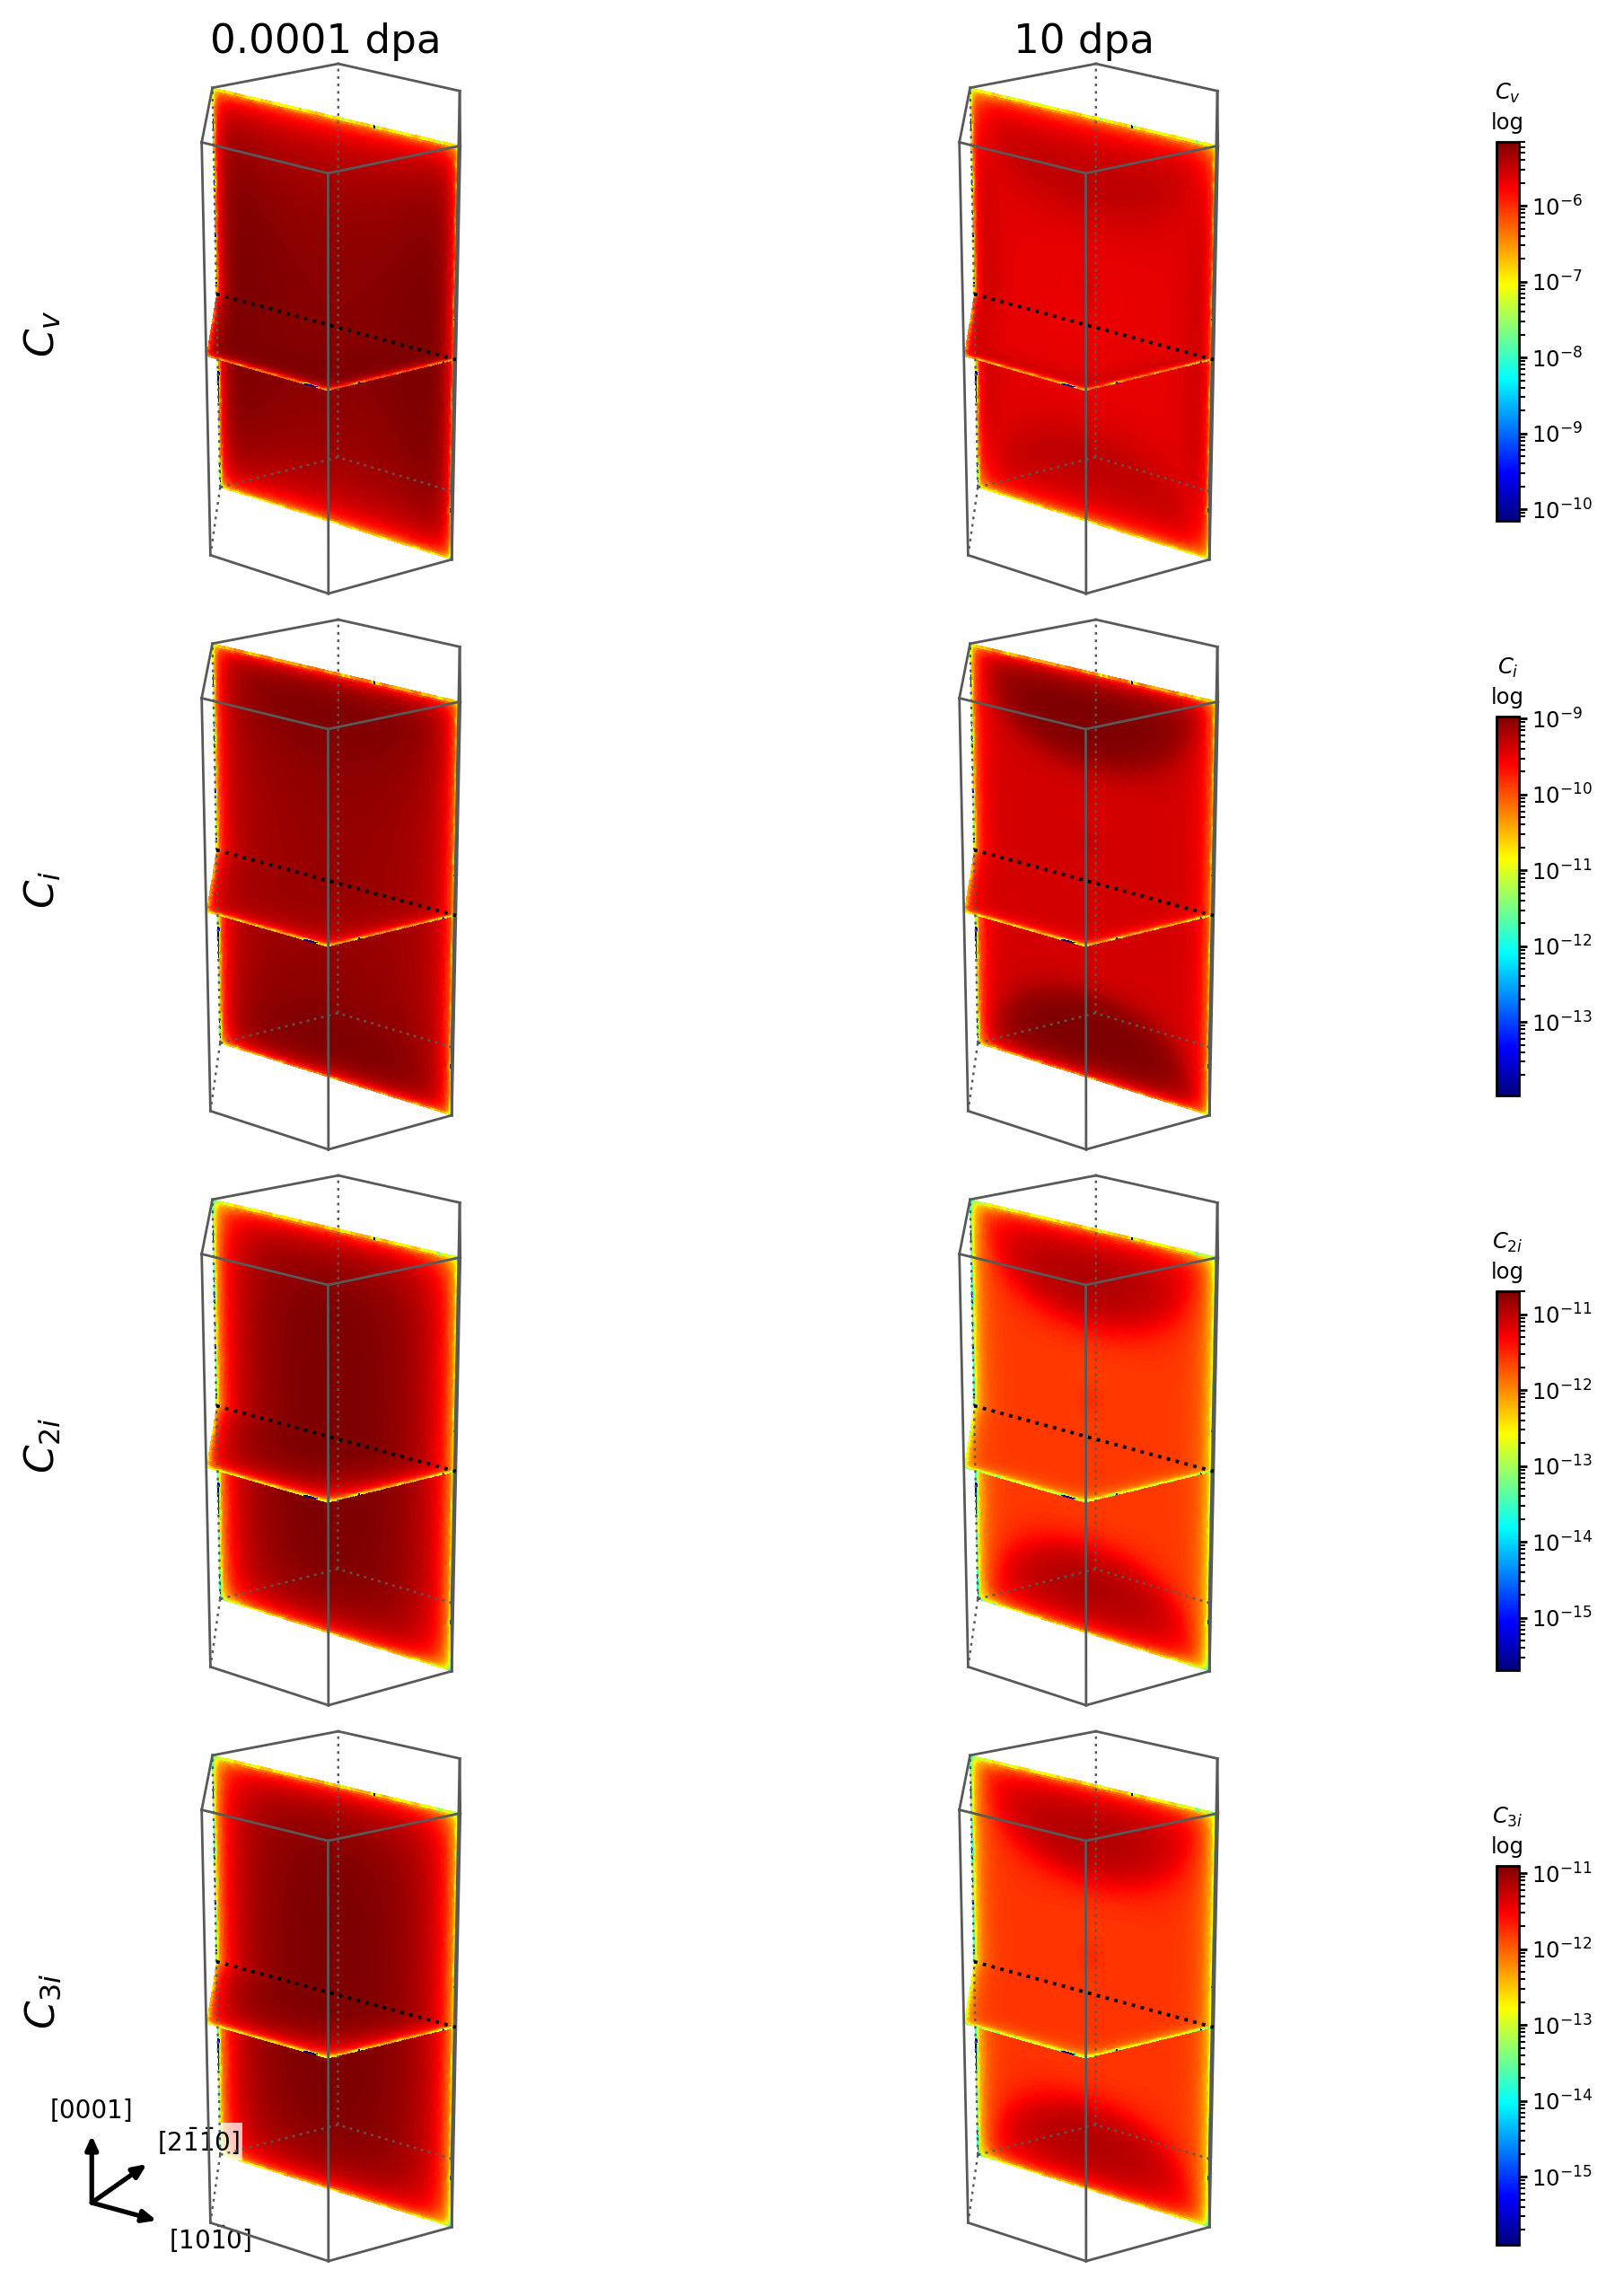
\includegraphics[width=\textwidth]{figures/mobile_early_late.png}
\caption{Mobile species at $10^{-4}\,$dpa (left) and 10\,dpa (right), on one
vertical and one horizontal mid-cut. Rows, top to bottom: $C_v$, $C_i$,
$C_{2i}$, $C_{3i}$; each row has its own logarithmic color scale, so levels are
comparable across dose within a row and not between rows. The interior plateau
falls and the depleted shell narrows between the two doses, both because the
sink density has risen.}
\label{fig:mobile}
\end{figure}

\paragraph{The boundary layer is a diffusion length and it orders the species.}
Measuring the layer as the distance at which the binned median recovers
$1-e^{-1}$ of the interior plateau:

\begin{center}
\begin{tabular}{@{}lrrrr@{}}
\toprule
Dose (dpa) & $C_v$ & $C_i$ & $C_{2i}$ & $C_{3i}$ \\
\midrule
$10^{-4}$ & 16.5\,nm & 27.5\,nm & 46.0\,nm & 46.0\,nm \\
$10^{-2}$ & 14.9\,nm & 27.5\,nm & 46.0\,nm & 46.0\,nm \\
$10$      &  8.0\,nm & 16.5\,nm & 18.2\,nm & 18.2\,nm \\
\bottomrule
\end{tabular}
\end{center}

Two readings, and both are consequences of $L\sim\sqrt{D/k^{2}}$ rather than of
anything fitted. \emph{Across species at fixed dose}, the layer widens with
mobility: the vacancy, least mobile, is depleted over the shortest distance,
while the interstitial clusters --- which reach a sink from further away ---
carry the widest layer. \emph{Across dose at fixed species}, every layer
narrows, by a factor of two between $10^{-4}$ and 10\,dpa, because $k^{2}$ has
grown with the loop population that the same calculation is building. The
boundary layer is therefore not a fixed geometric feature of the domain; it is a
running measure of the sink density, and it tightens as the microstructure
develops.

\paragraph{Anisotropy acts on the shape of the layer, not only its width.}
Because the domain has two basal faces and six prismatic ones, the layer can be
measured separately toward each set, using only the nodes for which that set is
the nearer boundary:

\begin{center}
\begin{tabular}{@{}lrrrr@{}}
\toprule
& \multicolumn{2}{c}{$10^{-4}$\,dpa} & \multicolumn{2}{c}{10\,dpa} \\
\cmidrule(lr){2-3}\cmidrule(lr){4-5}
Species & toward basal & toward prismatic & toward basal & toward prismatic \\
\midrule
$C_v$    & 84.8\,nm & 11.7\,nm & 24.0\,nm & 6.8\,nm \\
$C_i$    & 12.8\,nm & 28.8\,nm &  7.5\,nm & 18.3\,nm \\
$C_{2i}$ & 22.0\,nm & 45.2\,nm &  6.8\,nm & 24.0\,nm \\
$C_{3i}$ & 24.0\,nm & 45.2\,nm &  6.8\,nm & 24.0\,nm \\
\bottomrule
\end{tabular}
\end{center}

The vacancy layer is $7.2$ times \emph{wider} toward the basal faces than toward
the prismatic ones, which is the sign the fitted $p^{v}=1.6$ requires: vacancies
are $16.8$ times more mobile along $[0001]$ (\cref{eq:Dratio}), and a species
that reaches a sink from further away is depleted over a longer distance. The
scale expected from $L\sim\sqrt{D/k^{2}}$ is
$\sqrt{16.8}=4.1$, so the measured $7.2$ is not a clean reading of the
diffusivity ratio, and the interstitial rows show why. At $p^{i}=1.0$ the
interstitials diffuse isotropically, yet their layer is \emph{narrower} toward
the basal faces by a factor of $0.44$ --- an effect of domain shape rather than
of transport, since a node near a prismatic face is close to several faces at
once and is depleted more than its distance to the nearest one would suggest.
Anisotropy and geometry therefore act in opposite directions here, and only
their combination is directly observable.

Two consequences. First, an SRCD calculation on a shaped grain measures the
convolution of the diffusion tensor with the grain geometry, so extracting one
requires the other to be known --- which is an argument for calibrating $p^{m}$
atomistically rather than from a boundary-layer profile
(\cref{sec:conclusions}). Second, the narrowest layer in the problem is the
interstitial one toward a basal face, $7.5\,$nm at 10\,dpa, against a
$20\,$nm boundary element: the steepest gradient the calculation contains is
resolved by well under one element, and it is at exactly such a location that an
earlier calculation on this geometry drove a single node beyond the integrator's
reach (\cref{sec:failure}).

Interior median concentrations fall over the march --- $C_v$ from
$6.02\times10^{-6}$ to $2.29\times10^{-6}$, $C_i$ from $7.92\times10^{-10}$ to
$4.16\times10^{-10}$, and the clusters by nearly an order of magnitude --- which
is the signature of a rising sink density at constant production.

\subsection{Immobile fields and their moments}
\label{sec:results-moments}

\Cref{fig:moments-cf,fig:moments-a1} show the three carried moments of the
faulted basal family and of one prismatic interstitial variant, at the same two
doses. The three rows are not three views of one thing; they answer different
questions, and their spatial structures differ.

\begin{figure}[htbp]
\centering
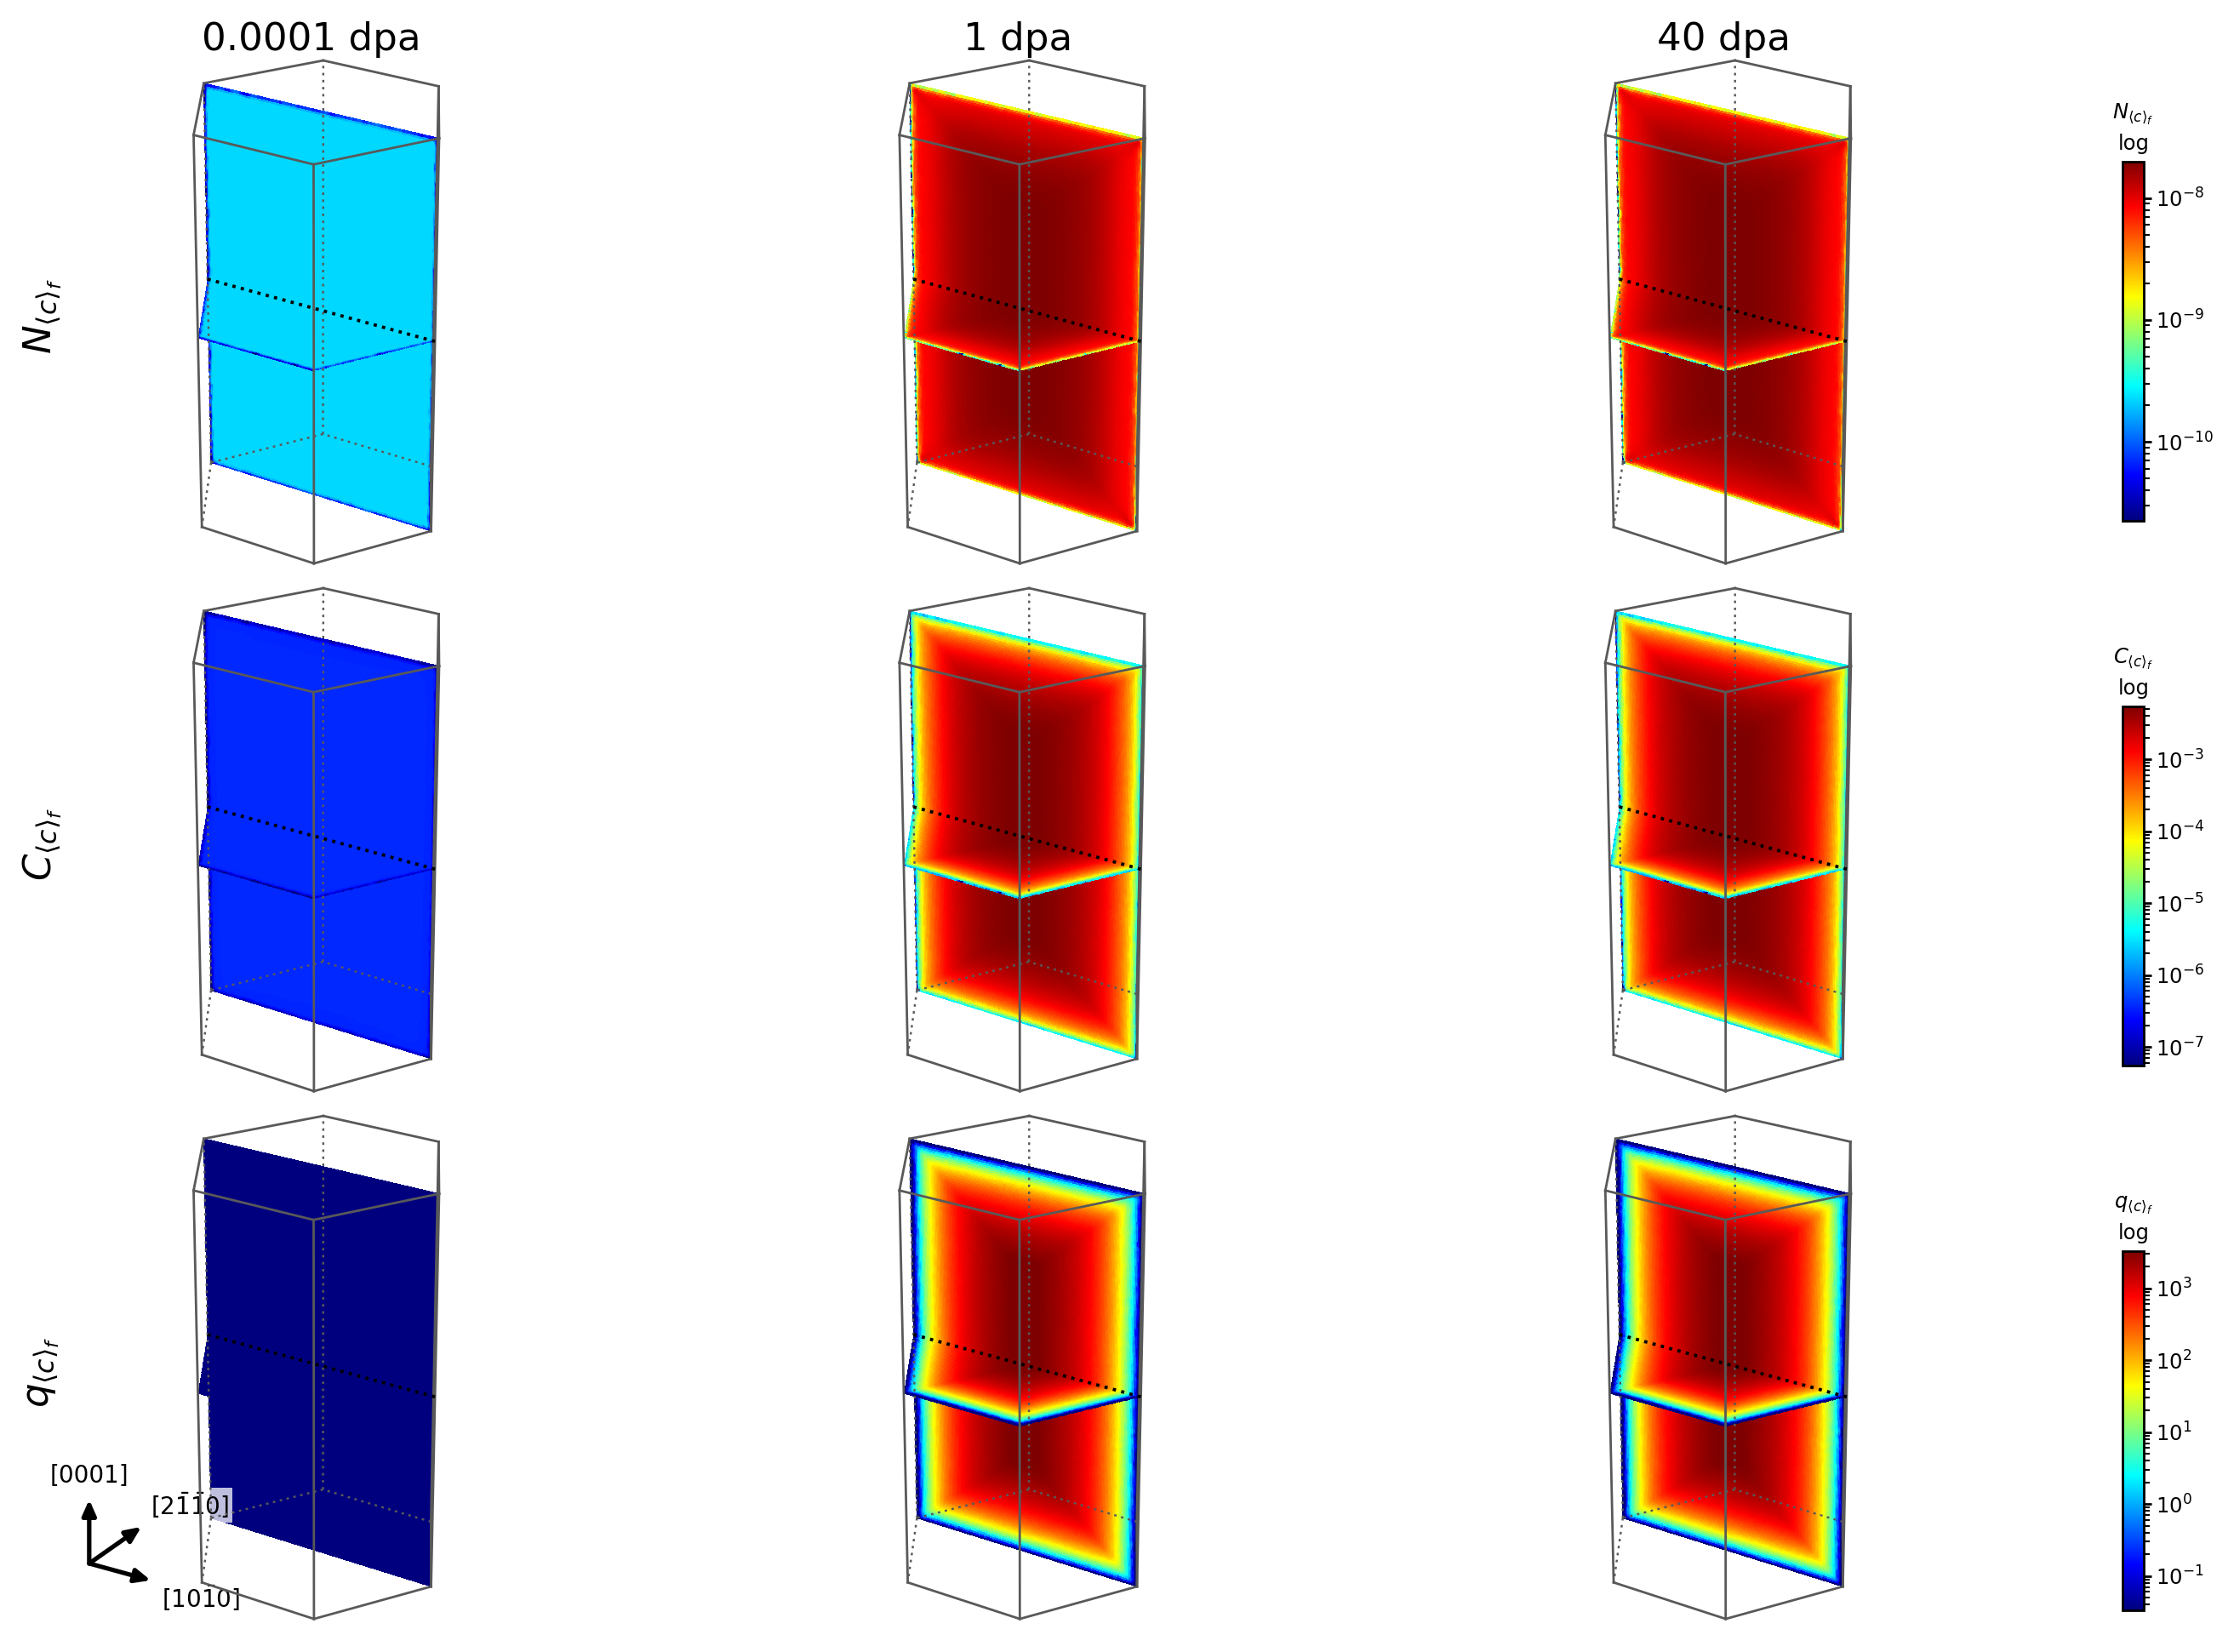
\includegraphics[width=\textwidth]{figures/moments_cf.png}
\caption{The basal faulted family $c_f$ at $10^{-4}$ and 10\,dpa: number density
$n$ (top), stored content $c$ (middle), second content $q$ (bottom).}
\label{fig:moments-cf}
\end{figure}

\begin{figure}[htbp]
\centering
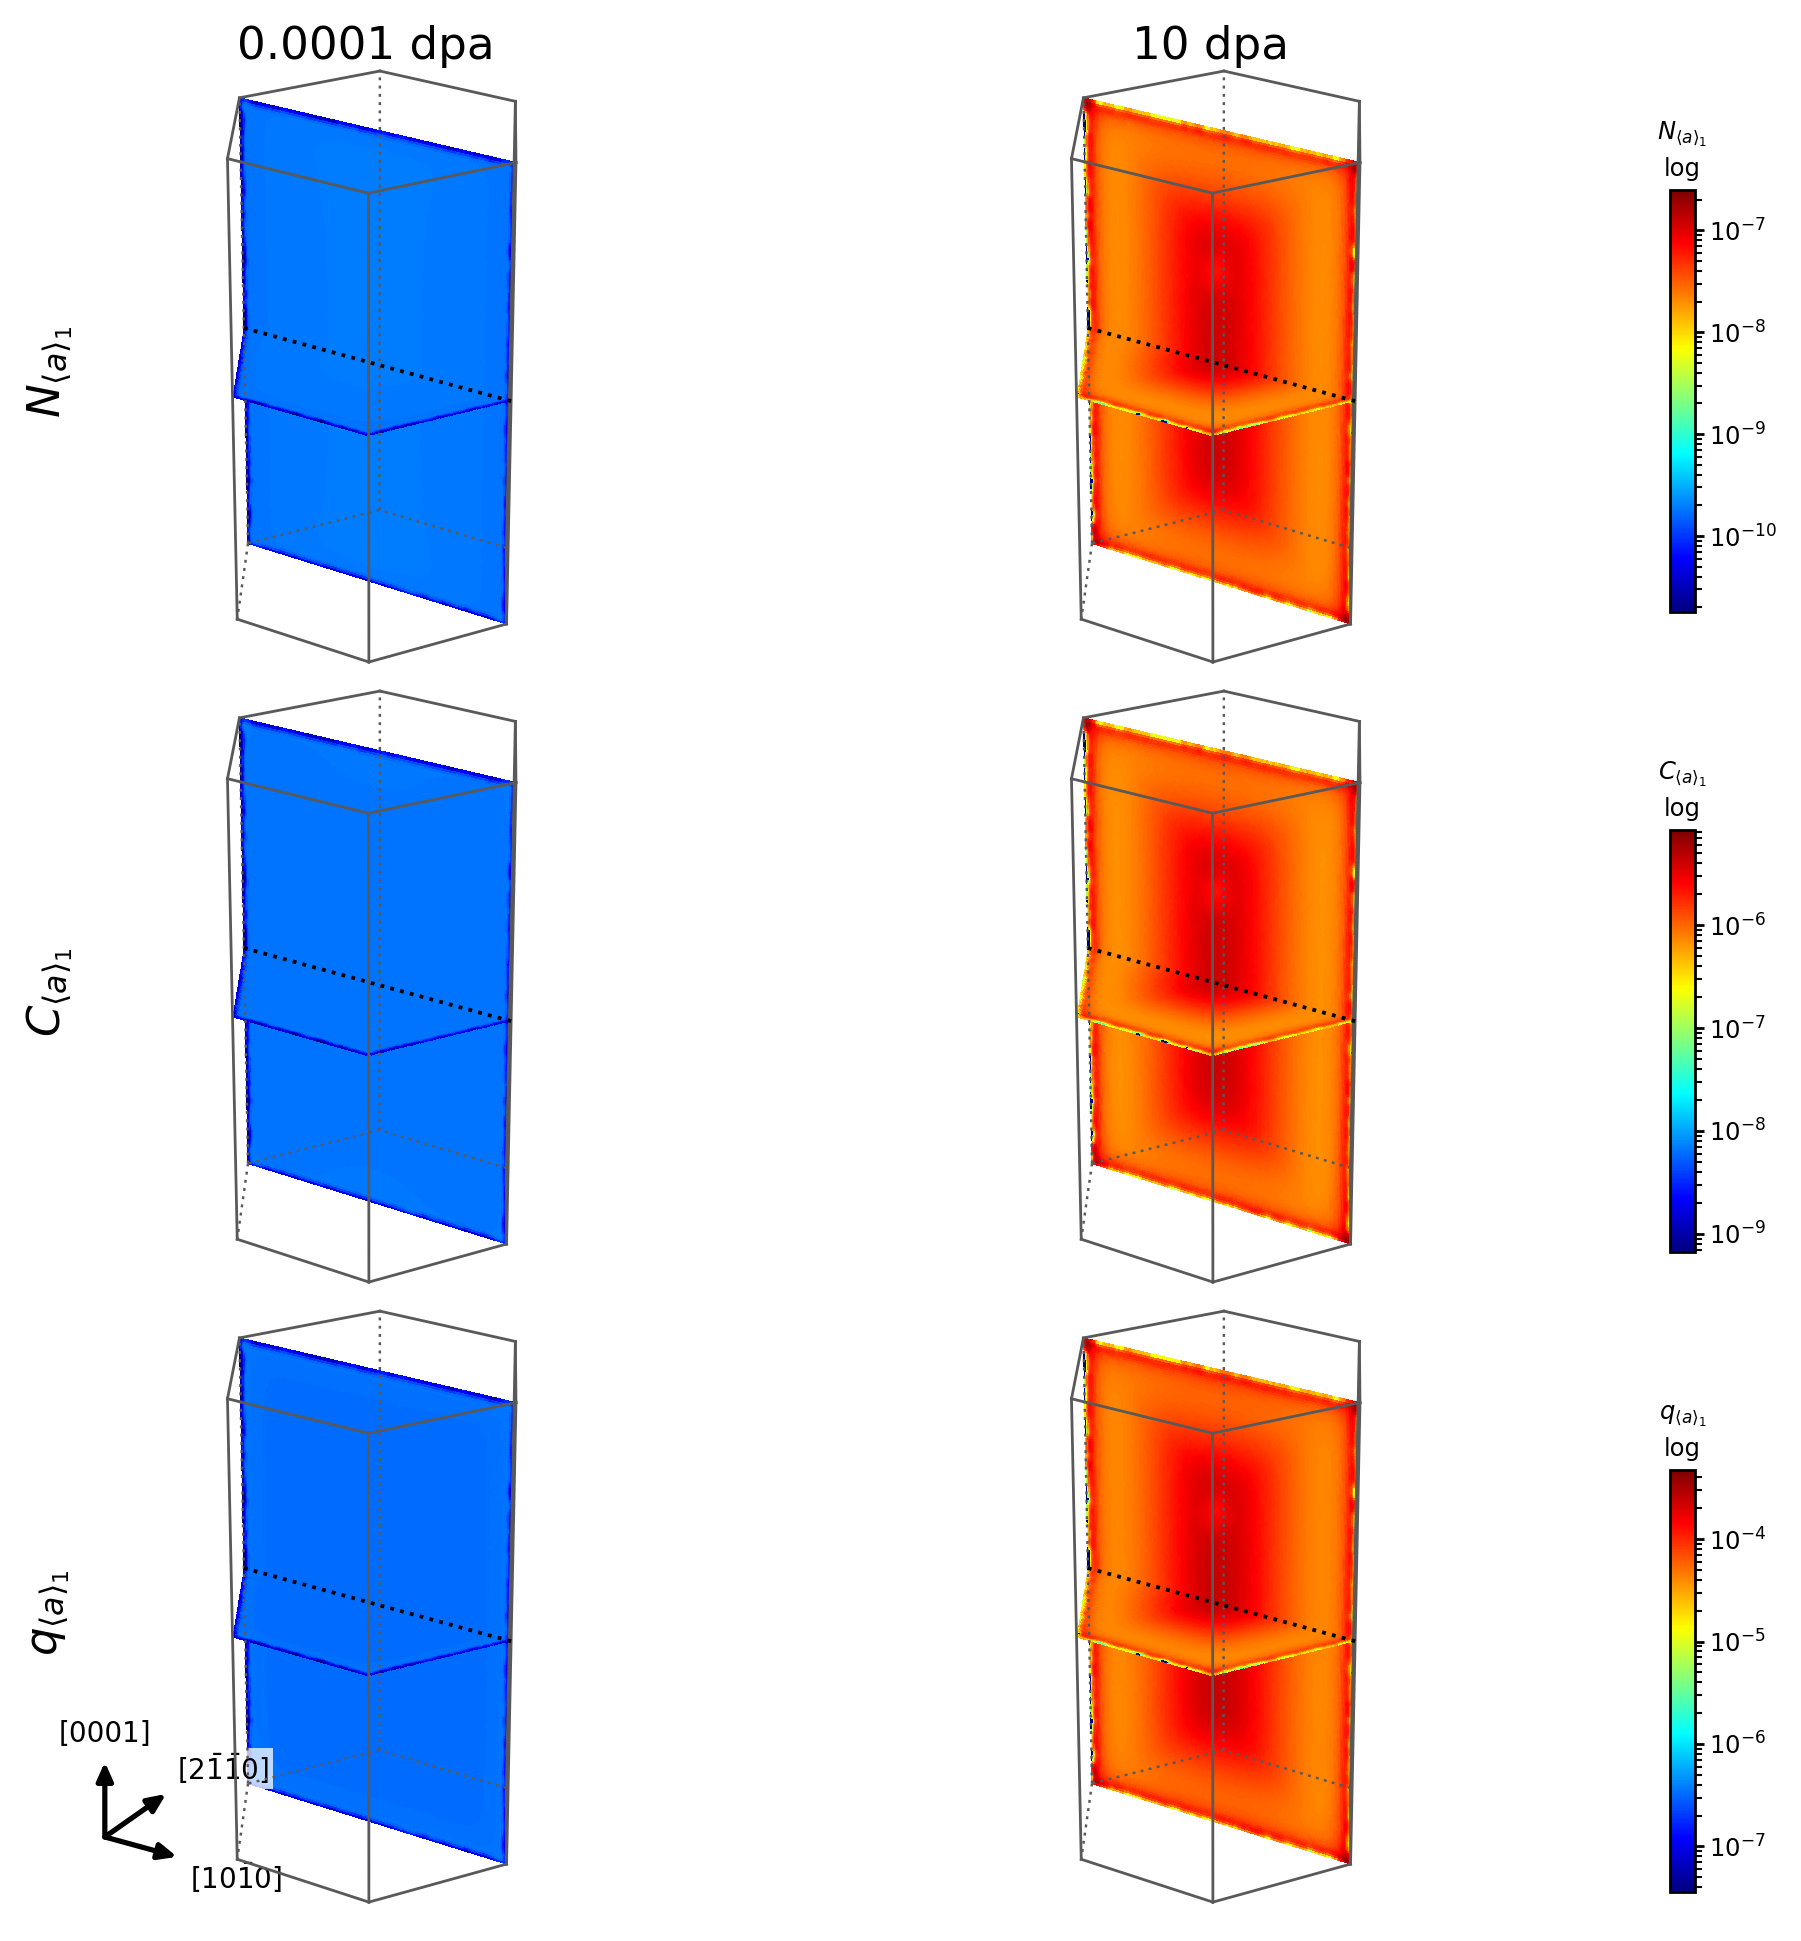
\includegraphics[width=\textwidth]{figures/moments_a1.png}
\caption{The prismatic interstitial variant $a_1$ at the same two doses, same
three moments. The variants $a_2$ and $a_3$ are identical at zero applied
stress and are not shown.}
\label{fig:moments-a1}
\end{figure}

\paragraph{Number is boundary-peaked, content is interior-peaked, and that is
the physics.} Cascade nucleation is spatially uniform, but the only channel that
removes a loop in the interior is coalescence, whose rate is driven by the
absorbed mobile flux --- and that flux vanishes where the Dirichlet condition
pins the mobile species. Near a boundary, loops are therefore nucleated and not
removed, so $n$ rises steeply toward the surface. They are also not \emph{fed},
because the same vanishing flux is what would grow them, so $c$ does not rise
with $n$ and the mean size $c/n$ collapses. Without the channel of
\cref{sec:gb-loops} that shell dominates every domain average, which is the
artifact \cref{sec:results-volume} quantifies.

\paragraph{The second moment does work, and it is realizable everywhere.} The
dispersion $\Delta_k=q n/c^{2}$ of \cref{eq:lognormal} must be $\ge1$ for the
three carried numbers to be the moments of any distribution at all. Measured
over the interior:

\begin{center}
\begin{tabular}{@{}lrrrrrr@{}}
\toprule
& \multicolumn{2}{c}{$c_f$} & \multicolumn{2}{c}{$a_1$}
& \multicolumn{2}{c}{$a_1^{v}$} \\
\cmidrule(lr){2-3}\cmidrule(lr){4-5}\cmidrule(lr){6-7}
Dose (dpa) & median & min & median & min & median & min \\
\midrule
$10^{-4}$ & 1.003 & 1.001 & 1.002 & 1.001 & 1.001 & 1.001 \\
$10^{-2}$ & 1.473 & 1.098 & 1.883 & 1.090 & 1.509 & 1.076 \\
$1$       & 1.559 & 1.250 & 2.724 & 2.442 & 2.215 & 2.112 \\
$10$      & 1.585 & 1.266 & 2.705 & 2.439 & 2.175 & 2.104 \\
\bottomrule
\end{tabular}
\end{center}

Three things follow. At $10^{-4}\,$dpa every family is monodisperse to
three decimal places, as it must be --- the loops present are all fresh nuclei
deposited at $m^{\mathrm{nuc}}_k$. By 1\,dpa the prismatic distribution has
broadened to $\Delta=2.72$, i.e. $s=\sqrt{\ln\Delta}=1.00$, a log-normal a full
decade wide at $\pm1\sigma$: a model carrying only $n$ and $c$ would represent
that population by a single size. And $\Delta\ge1$ holds at \emph{every}
interior node at every dose, minimum 1.001, which is the check that the channels
debiting $q$ are consistent with those debiting $n$ and $c$ --- a check that no
tolerance can substitute for, since $\Delta<1$ is not an inaccuracy but a
statement that the state is not a moment triple.

The basal family broadens less than the prismatic one ($1.59$ against $2.71$)
because its number loss is dominated by the boundary channel, which removes the
large end and therefore \emph{narrows} what remains, while the prismatic family
broadens under growth with no comparable truncation.

\subsection{Global conservation}
\label{sec:results-conservation}

The six atom-balance accumulators integrate the production, recombination and
sink absorption of each character, and the two accumulators of
\cref{sec:gb-loops} integrate the loop content taken by the boundary. In a
spatially resolved calculation on a Dirichlet domain the balance cannot close on
those channels alone, and the residual is not solver error: it is the atoms that
left through the surface as \emph{mobile} species. The magnitude settles the
matter --- nothing in an integration at $\mathrm{rtol}=10^{-6}$ is tens of
percent wrong.

\Cref{tab:conservation} is the balance over the whole march, per host atom.

\begin{table}[htbp]
\caption{The atom balance over $0\to10\,$dpa, volume-averaged, per host atom.
Production and recombination are exactly equal between the characters, as
Frenkel-pair production and recombination must be. The two channels that differ
are where the physics is: the network absorbs more interstitials than vacancies
(the bias), and the boundary absorbs vacancy \emph{loops} 60 times more than
interstitial ones.}
\label{tab:conservation}
\centering
\begin{tabular}{@{}lrrrr@{}}
\toprule
Channel & interstitial & vacancy & \%\,prod ($i$) & \%\,prod ($v$) \\
\midrule
produced                  & 10.0000 & 10.0000 & 100.00 & 100.00 \\
recombined                &  5.0832 &  5.0832 &  50.83 &  50.83 \\
absorbed at the network   &  0.7885 &  0.5908 &   7.88 &   5.91 \\
\textbf{loops at the boundary} & \textbf{0.0085} & \textbf{0.5123}
                          & \textbf{0.08} & \textbf{5.12} \\
stored in the microstructure & 0.0000 & 0.0020 & 0.00 & 0.02 \\
\midrule
mobile flux to the boundary (by difference)
                          &  4.1198 &  3.8117 &  41.20 &  38.12 \\
\bottomrule
\end{tabular}
\end{table}

Three readings.

\textbf{Both columns close on production.} $10.0000 = 5.0832+0.7885+0.0085+
0.0000+4.1198$ and likewise for the vacancies, so once the loop channel is
carried explicitly, what remains in the residual is the mobile flux alone and
the two do not contaminate each other. Before that channel was booked
separately, its 5.1\% of vacancy production was silently absorbed into the
residual, and because the residual is closure by difference, nothing looked
wrong.

\textbf{The boundary is the dominant sink, by a wide margin.} It takes
$41\%$ and $38\%$ of production as mobile species, against $7.9\%$ and $5.9\%$
at the network. That is a property of the geometry --- a 500\,nm grain with every
face absorbing --- and it is precisely what a mean-field model represents by a
single $k^{2}_{gb}$ and cannot resolve.

\textbf{The loop channel is strongly asymmetric.} It removes $0.512$ vacancies
per atom against $0.0085$ interstitials, a factor of 60. The asymmetry is
geometric, not biased: \cloop{} loops reach a mean radius of $25\,$nm where
\aloop{} loops reach $3\,$nm, so a basal loop intersects a face from far deeper
inside the crystal. Note also that the boundary removes \emph{250 times more}
vacancy loop content than the microstructure retains ($0.512$ against $0.0020$),
which is the quantitative form of the statement that on this grain size the
loop population is boundary-controlled.

\Cref{fig:conservation} shows the channels against dose and the fractional
decomposition. The fractions sum to unity once the boundary channels are
included; without them the sum reached only $\sim0.3$.

\begin{figure}[htbp]
\centering
\begin{minipage}{0.49\textwidth}\centering
  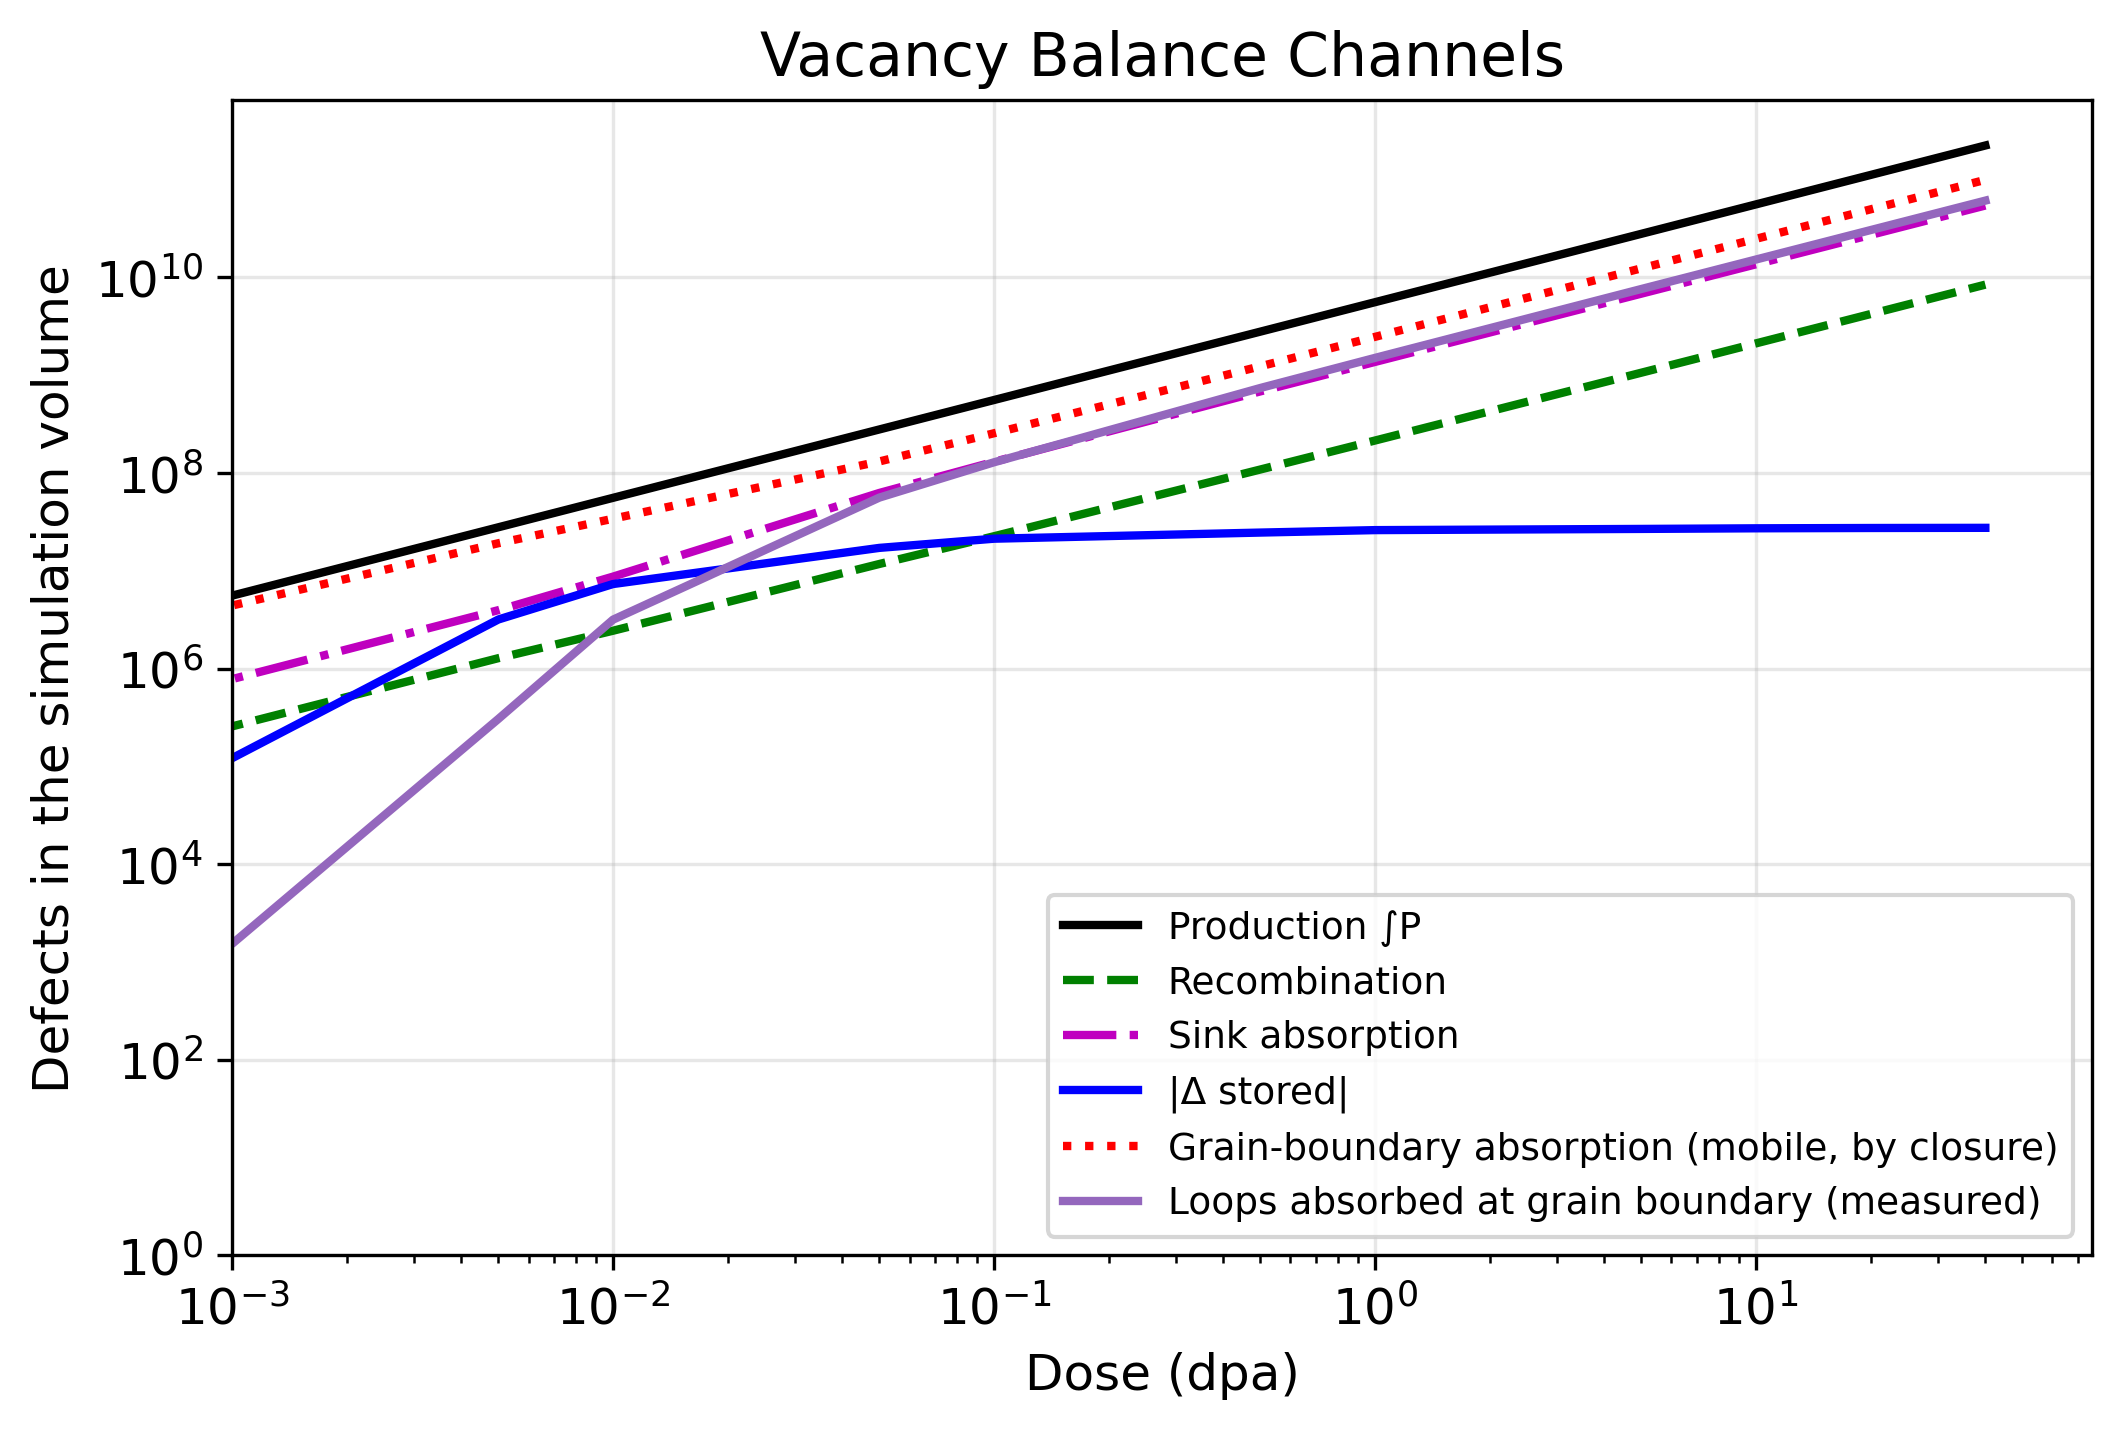
\includegraphics[width=\textwidth]{figures/conservation_v.png}
\end{minipage}\hfill
\begin{minipage}{0.49\textwidth}\centering
  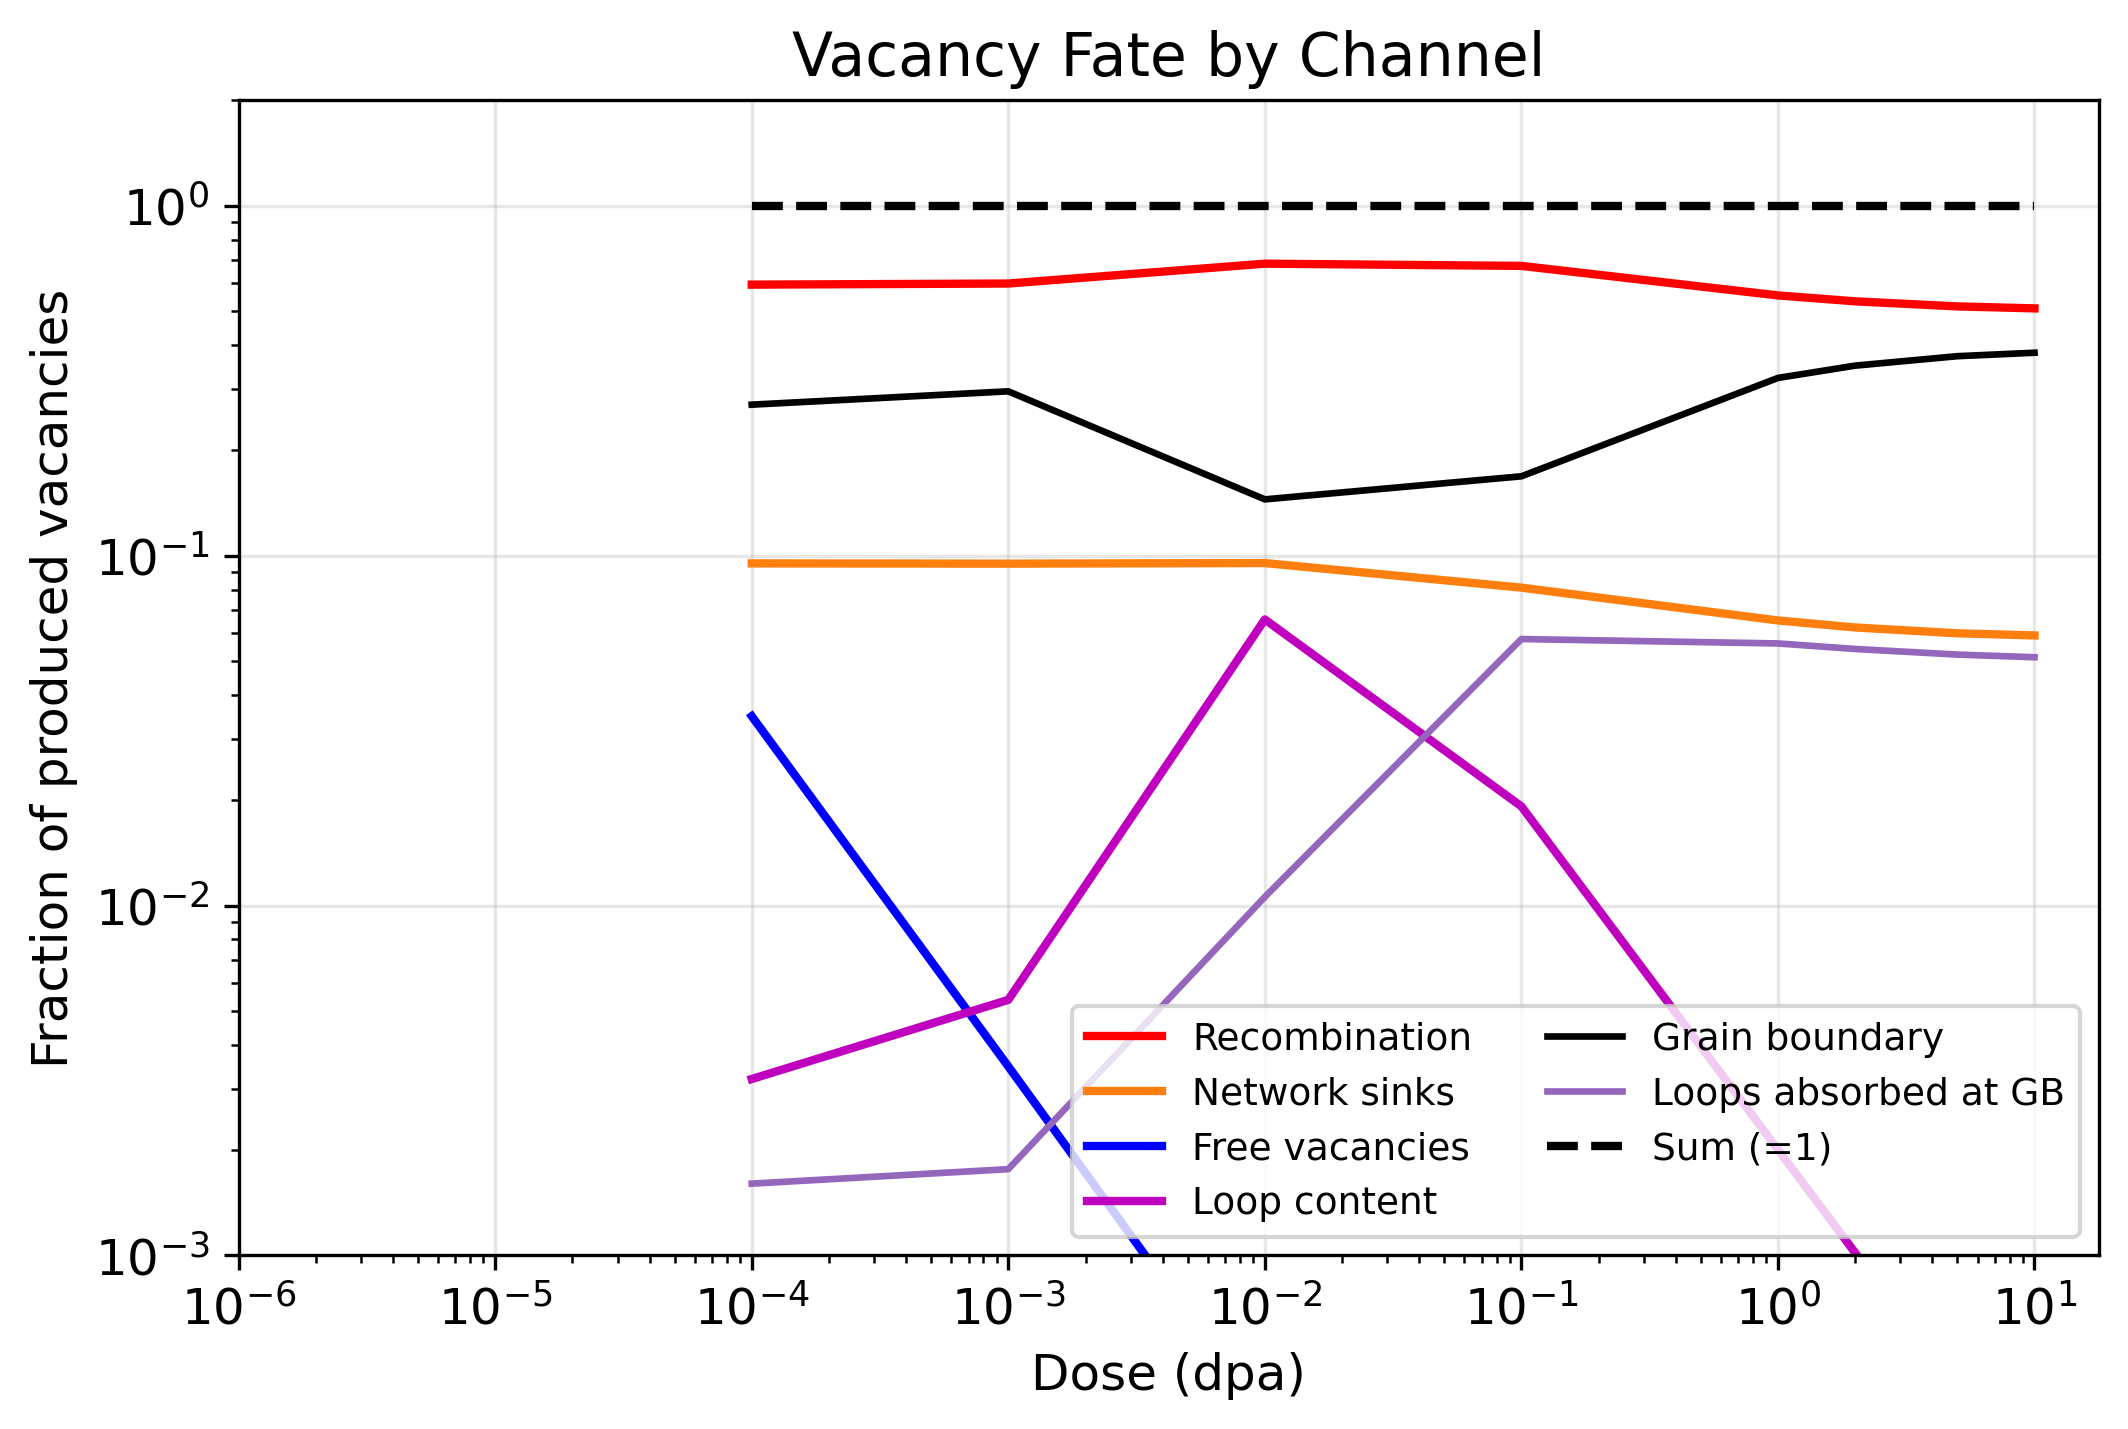
\includegraphics[width=\textwidth]{figures/fractions_v.png}
\end{minipage}
\caption{Vacancy balance against dose: cumulative channels (left) and their
fractions of production (right). The interstitial counterparts are similar
except that the loop-at-boundary channel is 60 times smaller.}
\label{fig:conservation}
\end{figure}

\begin{figure}[htbp]
\centering
\begin{minipage}{0.49\textwidth}\centering
  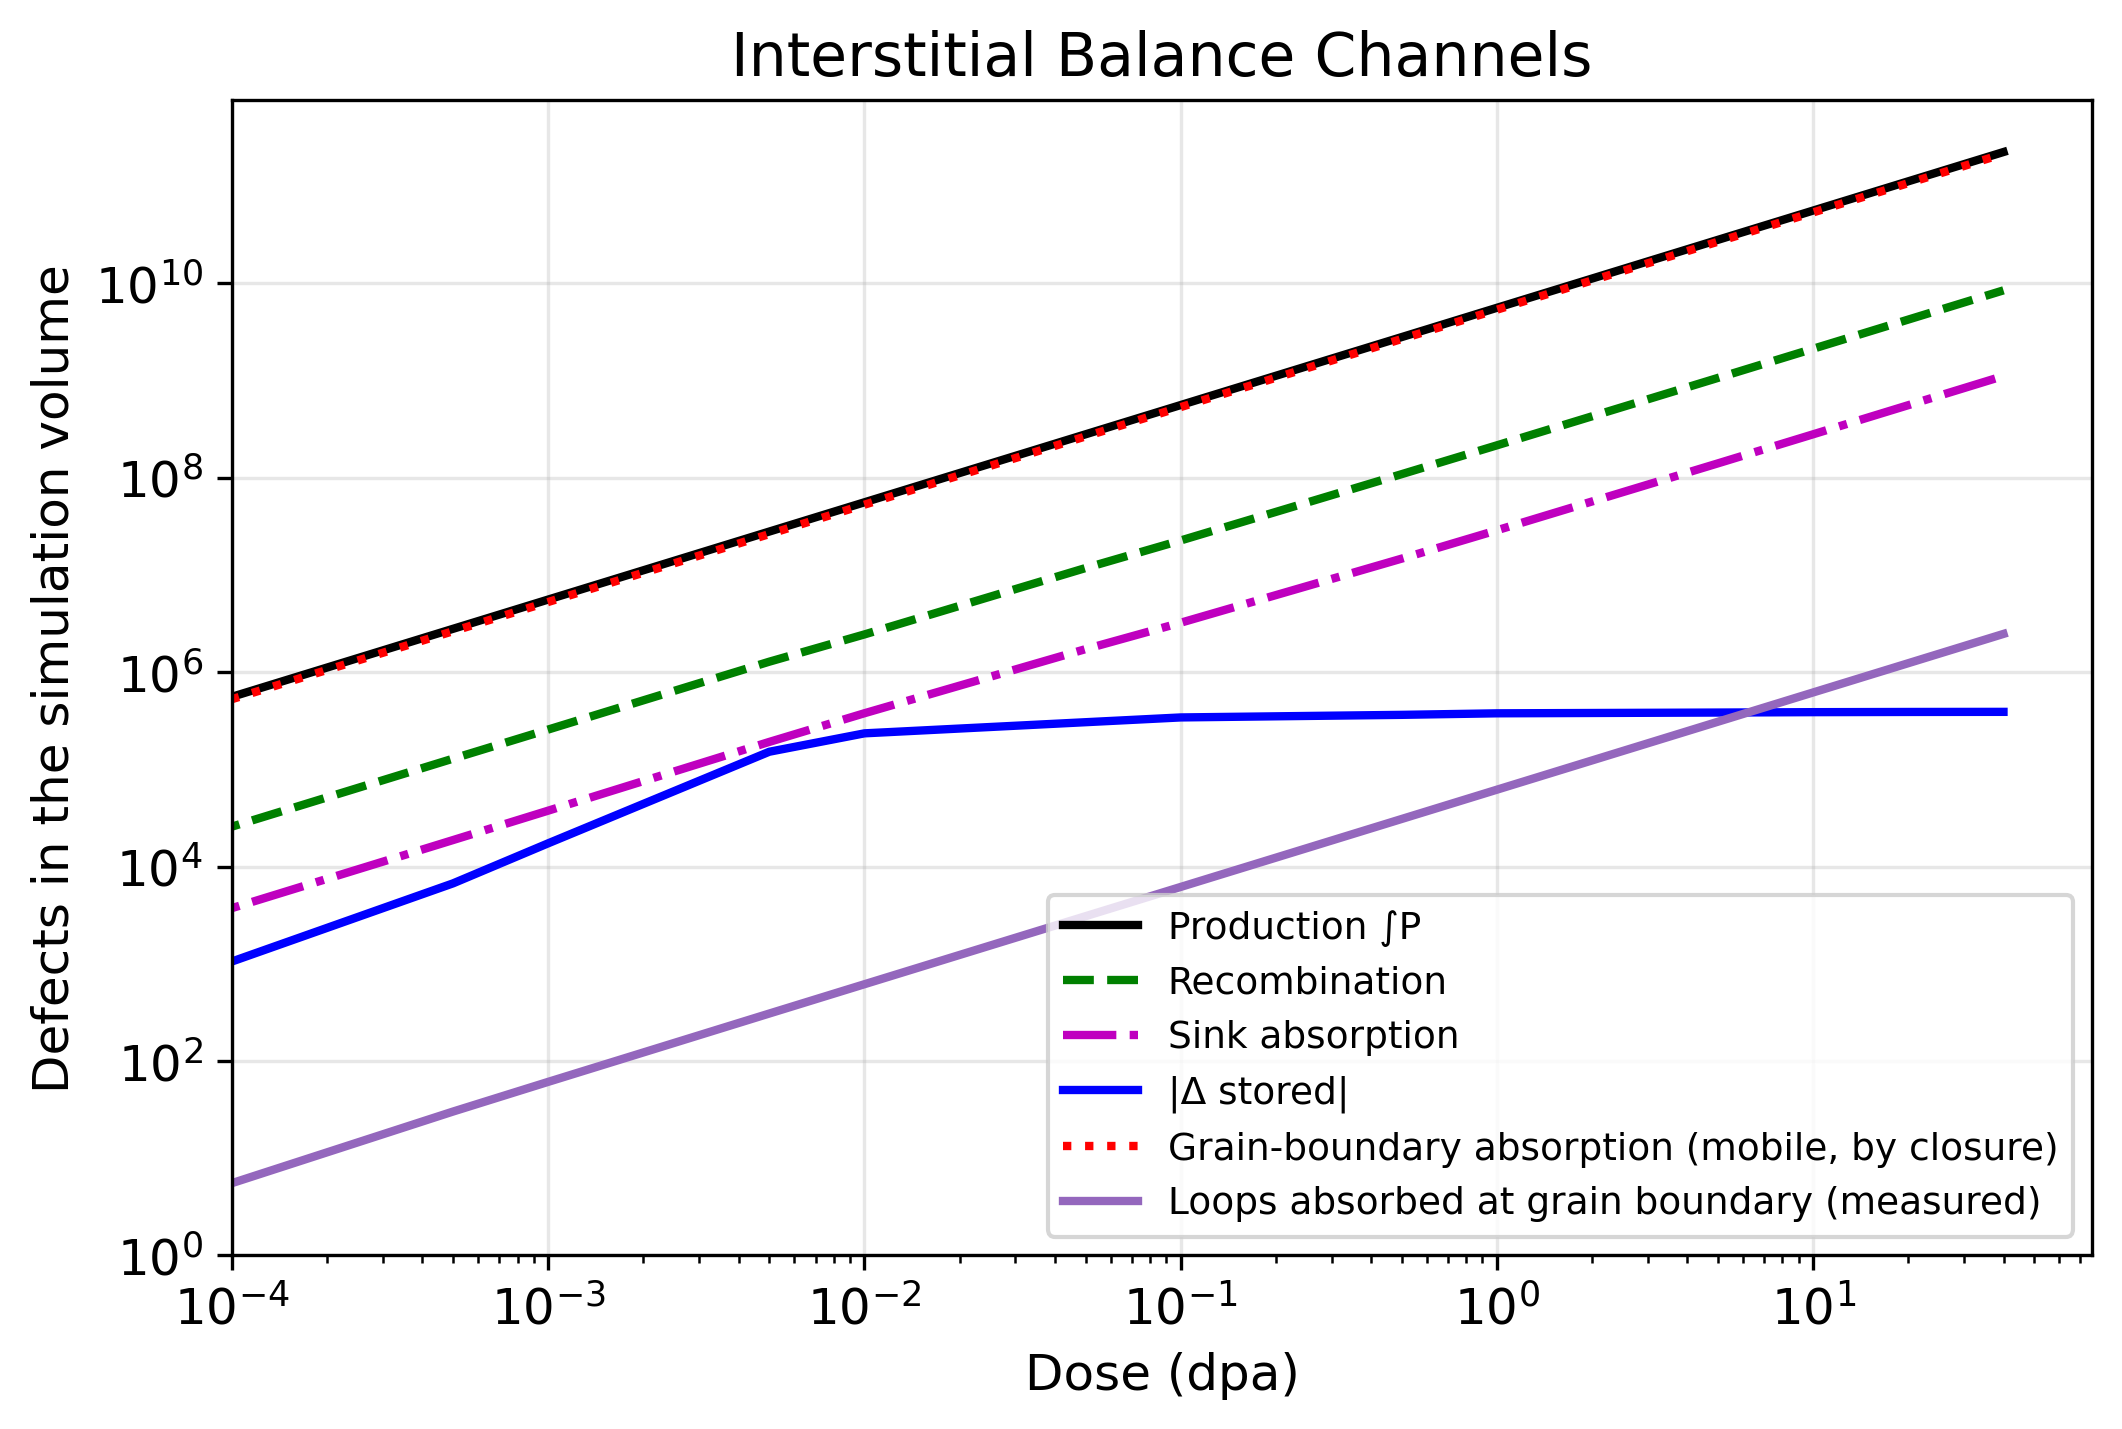
\includegraphics[width=\textwidth]{figures/conservation_i.png}
\end{minipage}\hfill
\begin{minipage}{0.49\textwidth}\centering
  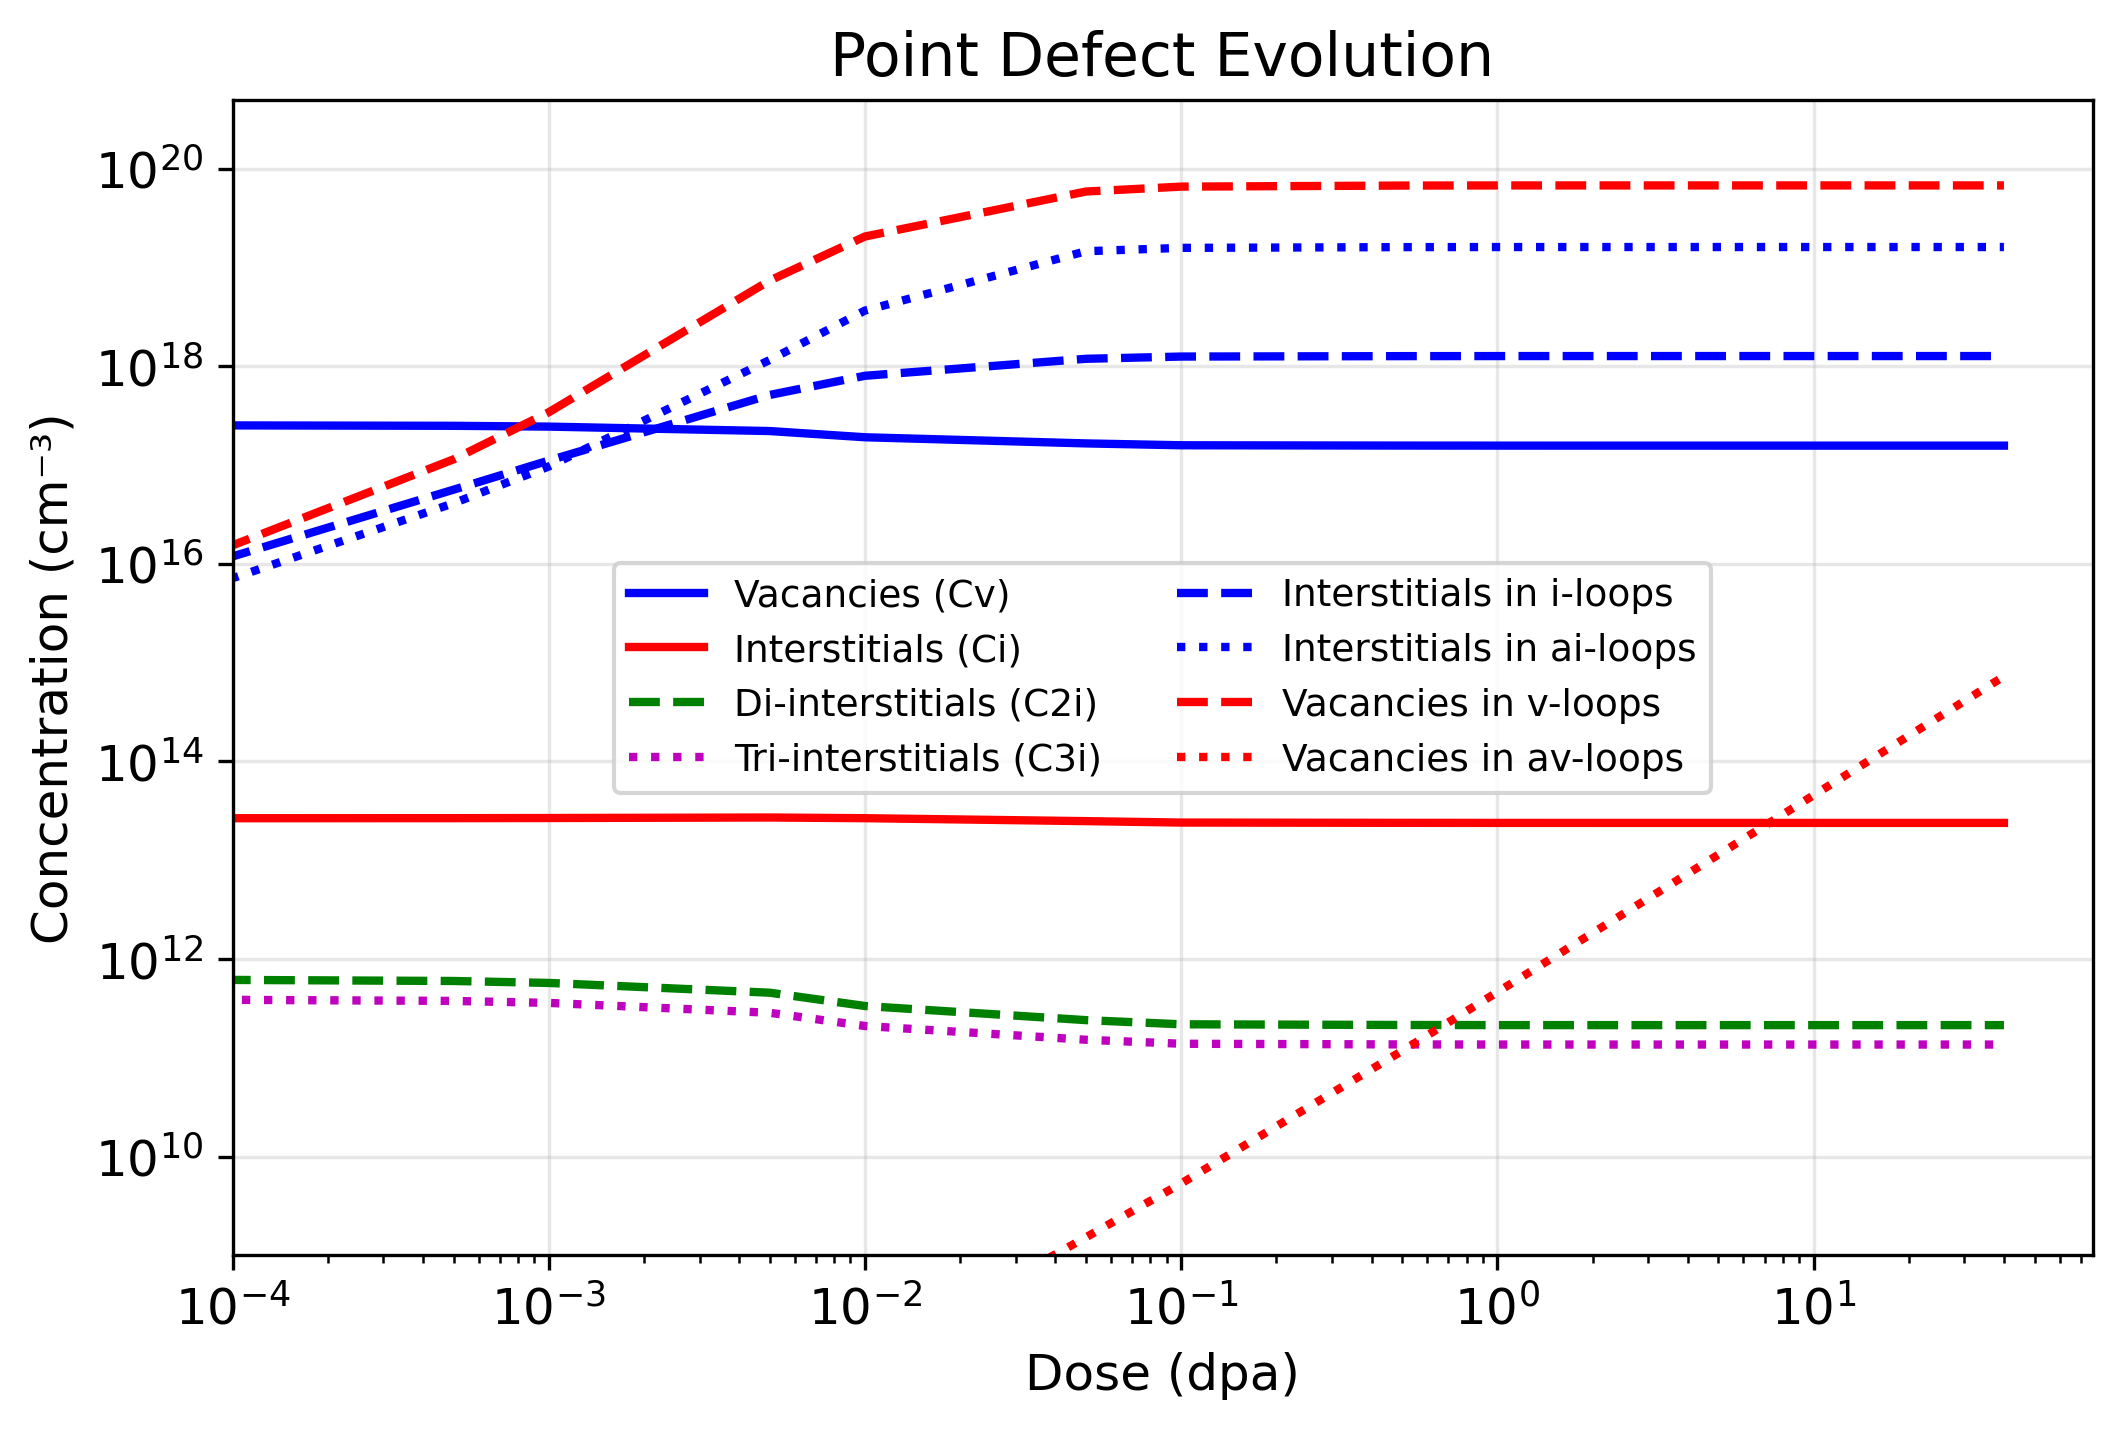
\includegraphics[width=\textwidth]{figures/point_defects.png}
\end{minipage}
\caption{Left: the interstitial balance against dose, the counterpart of
\cref{fig:conservation}. Right: the volume-averaged mobile concentrations, whose
fall through the march is the rising sink density of
\cref{sec:results-mobile} seen as an average rather than as a field.}
\label{fig:conservation-i}
\end{figure}

\subsection{Grain-boundary effects and the denuded zone}
\label{sec:results-gb}

\Cref{fig:denuded} is the central result of the loop channel: loop density and
mean diameter against distance to the nearest face, with and without it.

\begin{figure}[htbp]
\centering
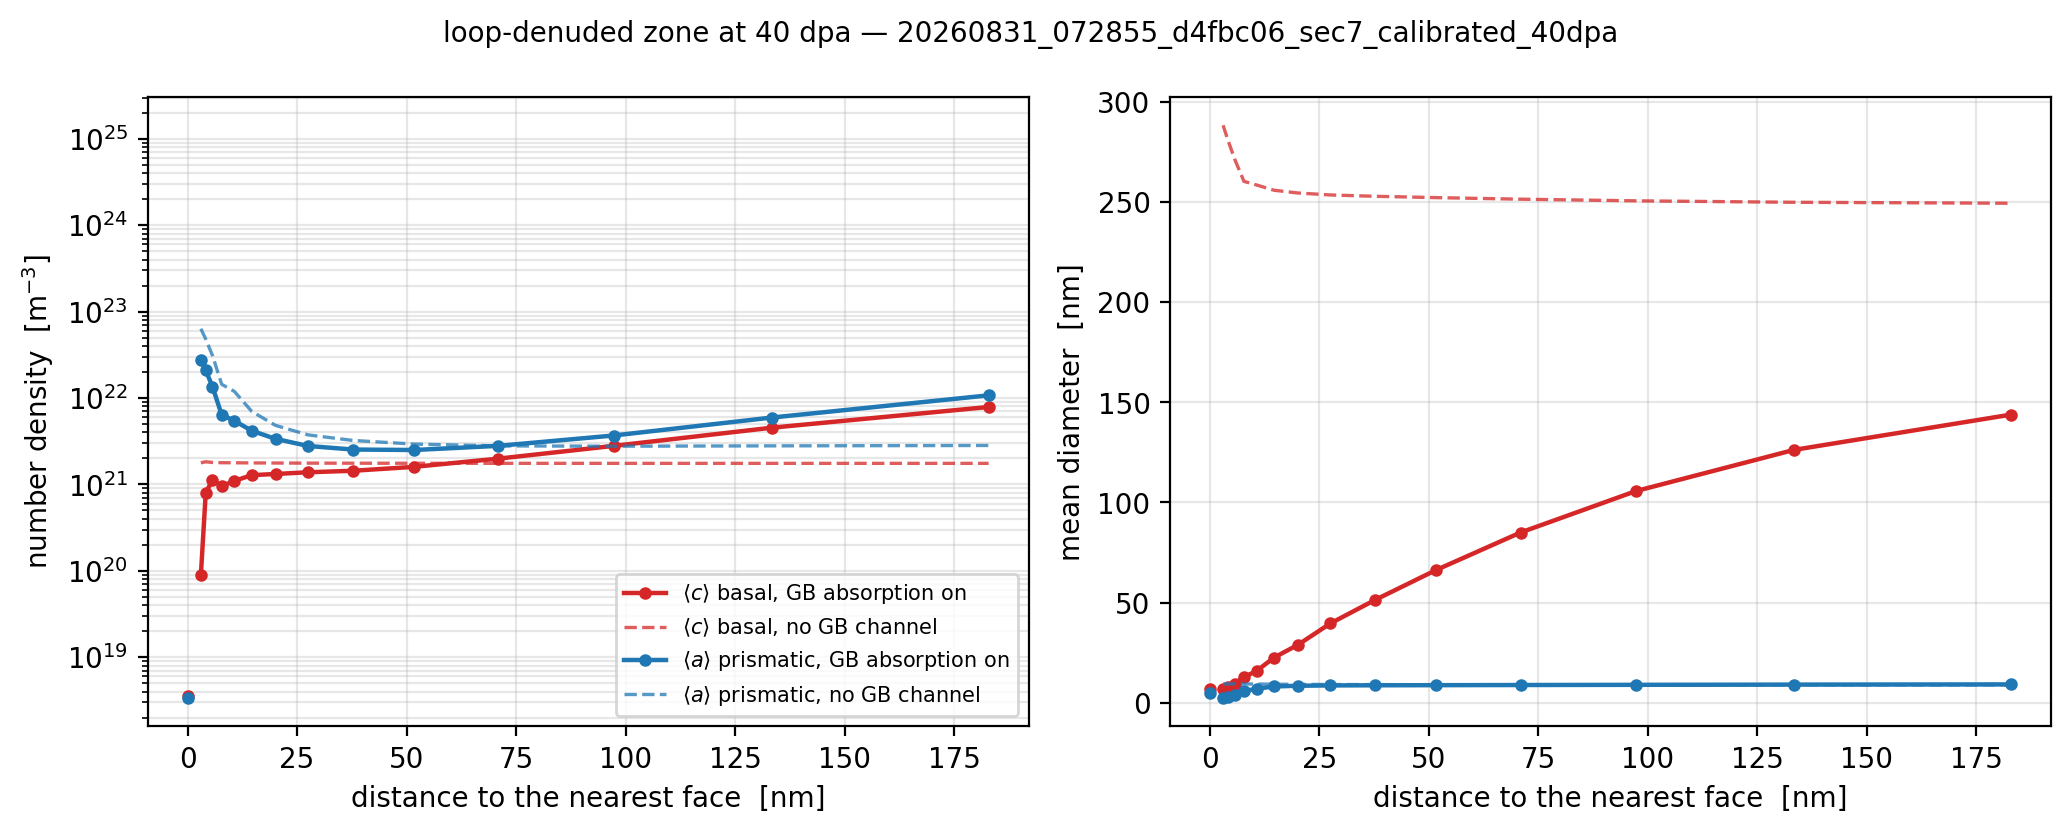
\includegraphics[width=\textwidth]{figures/denuded_zone.png}
\caption{The loop-denuded zone at 10\,dpa. Solid: grain-boundary loop absorption
active. Dashed: the identical calculation without it. Left, number density;
right, content-weighted mean diameter. The abscissa is the minimum distance to
any face, and the ordinate on the left is logarithmic over six decades.}
\label{fig:denuded}
\end{figure}

\begin{center}
\begin{tabular}{@{}lrrrr@{}}
\toprule
$x$ (nm) & $N_a$/twin & $N_c$/twin & $d_a$ (nm) & $d_c$ (nm) \\
\midrule
0--1        & $10^{-6}$ & $10^{-6}$ & 5.0 & 5.4 \\
3.5--4.9    & 0.646 & 0.608 & 4.6 & 3.5 \\
6.7--9.1    & 0.703 & 1.36  & 7.1 & 10.1 \\
23.6--32.3  & 2.95  & 5.45  & 5.7 & 32.5 \\
83.3--114.3 & 0.415 & 4.21  & 9.2 & 50.2 \\
156.8--215  & 0.670 & 12.6  & 8.9 & 57.9 \\
\bottomrule
\end{tabular}
\end{center}

\textbf{The zone is real, sharp, and about 5\,nm wide.} The face layer is swept
to $10^{-6}$ of the companion calculation --- which is the concentration floor,
so as complete a removal as this model can express --- and the depletion is still
measurable at 5--9\,nm. Beyond that the profile is no longer denuded. The mean
diameter recovers monotonically from $3.5\,$nm at the boundary to $58\,$nm in
the interior, which is the size gradient a denuded zone is identified by in a
micrograph: not merely fewer loops near the boundary, but \emph{smaller} ones,
because the large end of the distribution is what \cref{eq:gbloop} removes first.

\textbf{The ledger and the density profile measure different things, and both
are correct.} Of the total absorption, only 1.7\% occurs within 2\,nm of a face
and 93\% between 5 and 100\,nm. That is not a contradiction of the profile
above: the face layer is swept within the first dose interval, so for 99\% of the
march there is nothing left there to absorb, while the region further in keeps
\emph{supplying} loops that grow into contact. The density says where loops are
absent; the ledger says where the flux into the boundary came from over the whole
history.

\textbf{A local channel with non-local consequences.} The interior \cloop{}
density is 4--5 times the companion calculation's at \emph{every} distance,
including 200\,nm from any face where \cref{eq:mgb} removes nothing. The cause
is the operator split working as intended: removing the shell's loops removes
their sink strength from \cref{eq:KL}, the fast solve returns a different mobile
field everywhere, and the interior responds to it. A model in which the boundary
were only a mean-field sink strength could not produce this, because the
boundary's effect on the interior would be a single number rather than a changed
field.

\paragraph{Comparison with experiment.} Loop-denuded and void-denuded zones at
grain boundaries are a standard observation in irradiated
metals~\citep{singh1973influence,bai2010efficient,sun2013situ,cheng2016grain}, and the mechanism
assumed here --- the boundary as a strong sink whose influence extends a
diffusion length into the grain --- is the standard interpretation. \textbf{We
do not compare quantitatively against a measured zone width in zirconium}: no
such measurement is in the data set of \cref{tab:targets}, and the width
predicted here (a few nm for \aloop{}, growing to tens of nm in the size
profile) is offered as a prediction rather than as a validated result. It is
also, at $2$--$5\,$nm for the prismatic family, comparable with the $20\,$nm
element size of the boundary layer, so the \aloop{} zone in particular is
under-resolved and its width should be treated as an upper bound set by the
mesh.

\begin{figure}[htbp]
\centering
\begin{minipage}{0.49\textwidth}\centering
  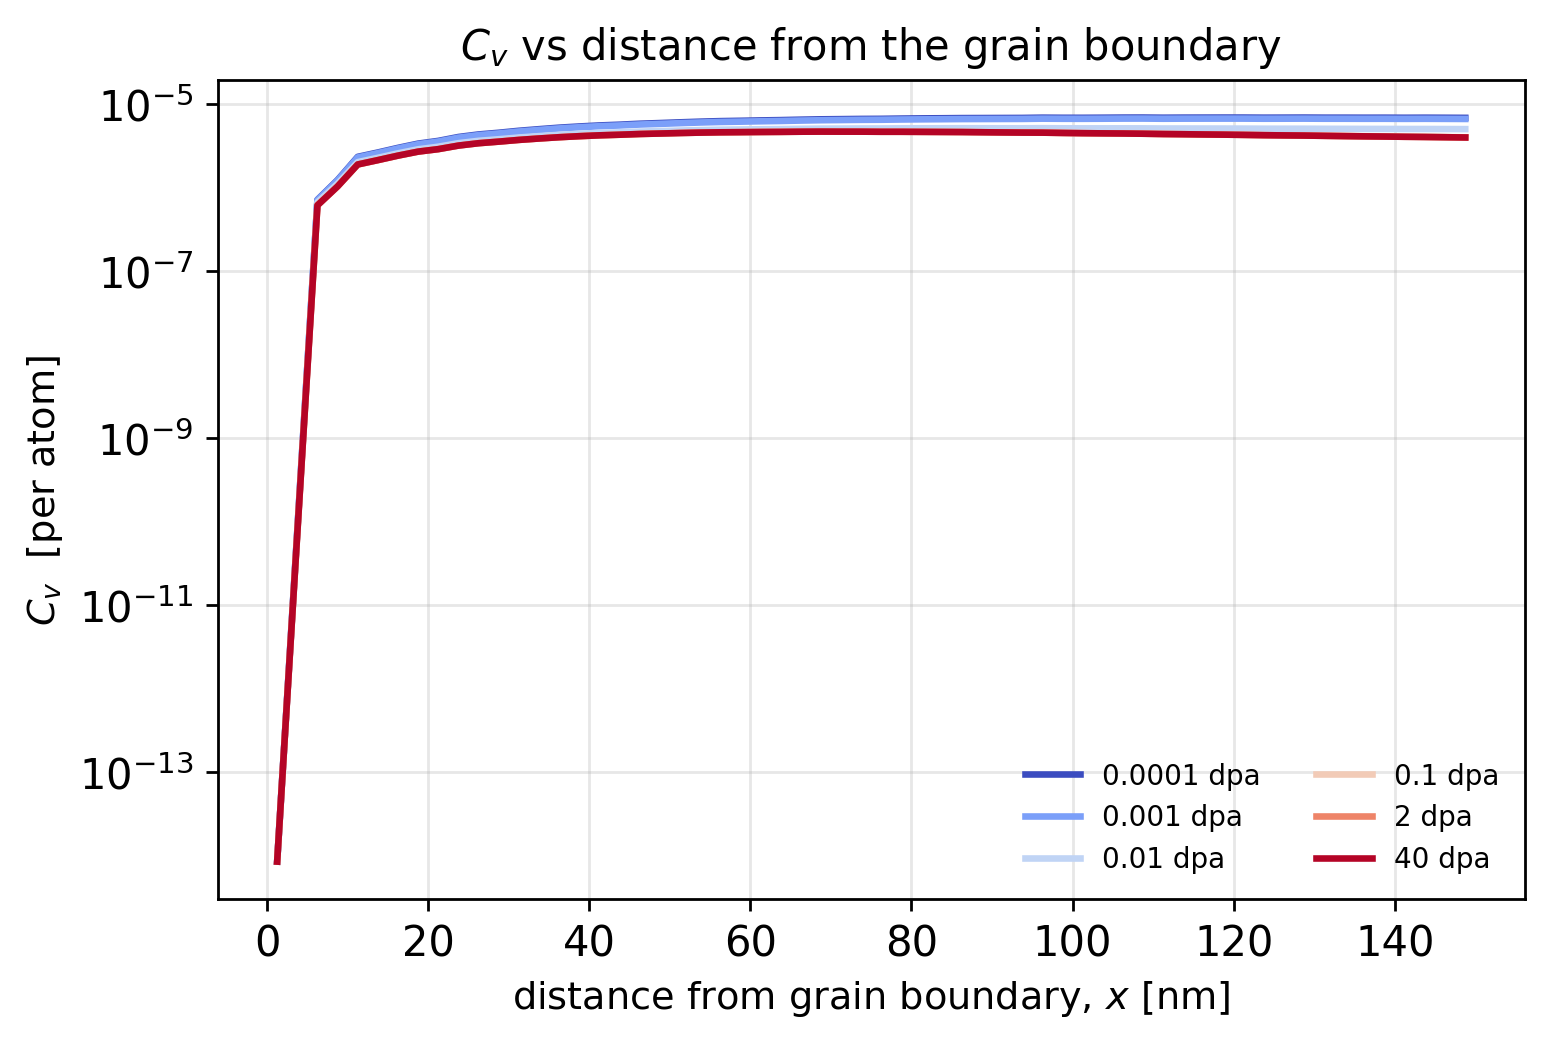
\includegraphics[width=\textwidth]{figures/gb_Cv.png}
\end{minipage}\hfill
\begin{minipage}{0.49\textwidth}\centering
  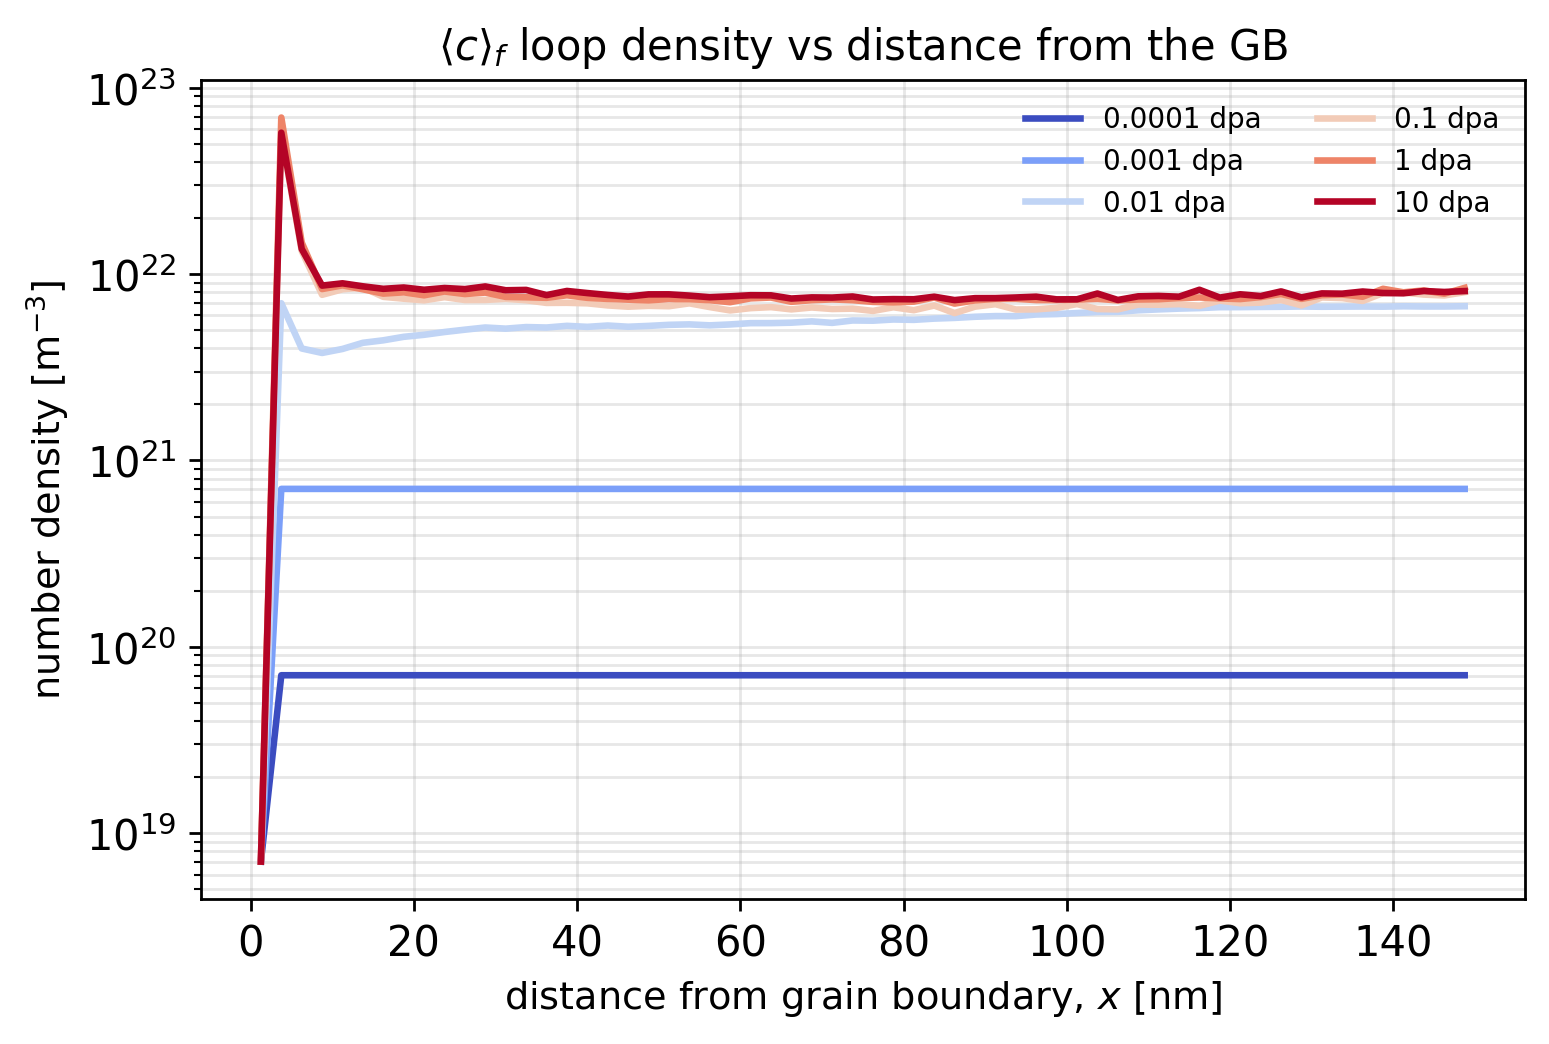
\includegraphics[width=\textwidth]{figures/gb_N_c.png}
\end{minipage}
\caption{Profiles against distance from the boundary over the first
\SI{150}{\nano\meter}, with every dose overlaid. Left: the mobile vacancy
concentration, whose recovery length is the boundary layer tabulated above and
which narrows as the dose accumulates. Right: the basal \cloop{} loop number
density, whose profile is the denuded zone of \cref{fig:denuded} seen at every
dose rather than only at the last.}
\label{fig:gb-profiles}
\end{figure}

\subsection{Volume averages and comparison with experiment}
\label{sec:results-volume}

\Cref{fig:volavg} shows the volume-averaged trajectories.

\begin{figure}[htbp]
\centering
\begin{minipage}{0.49\textwidth}\centering
  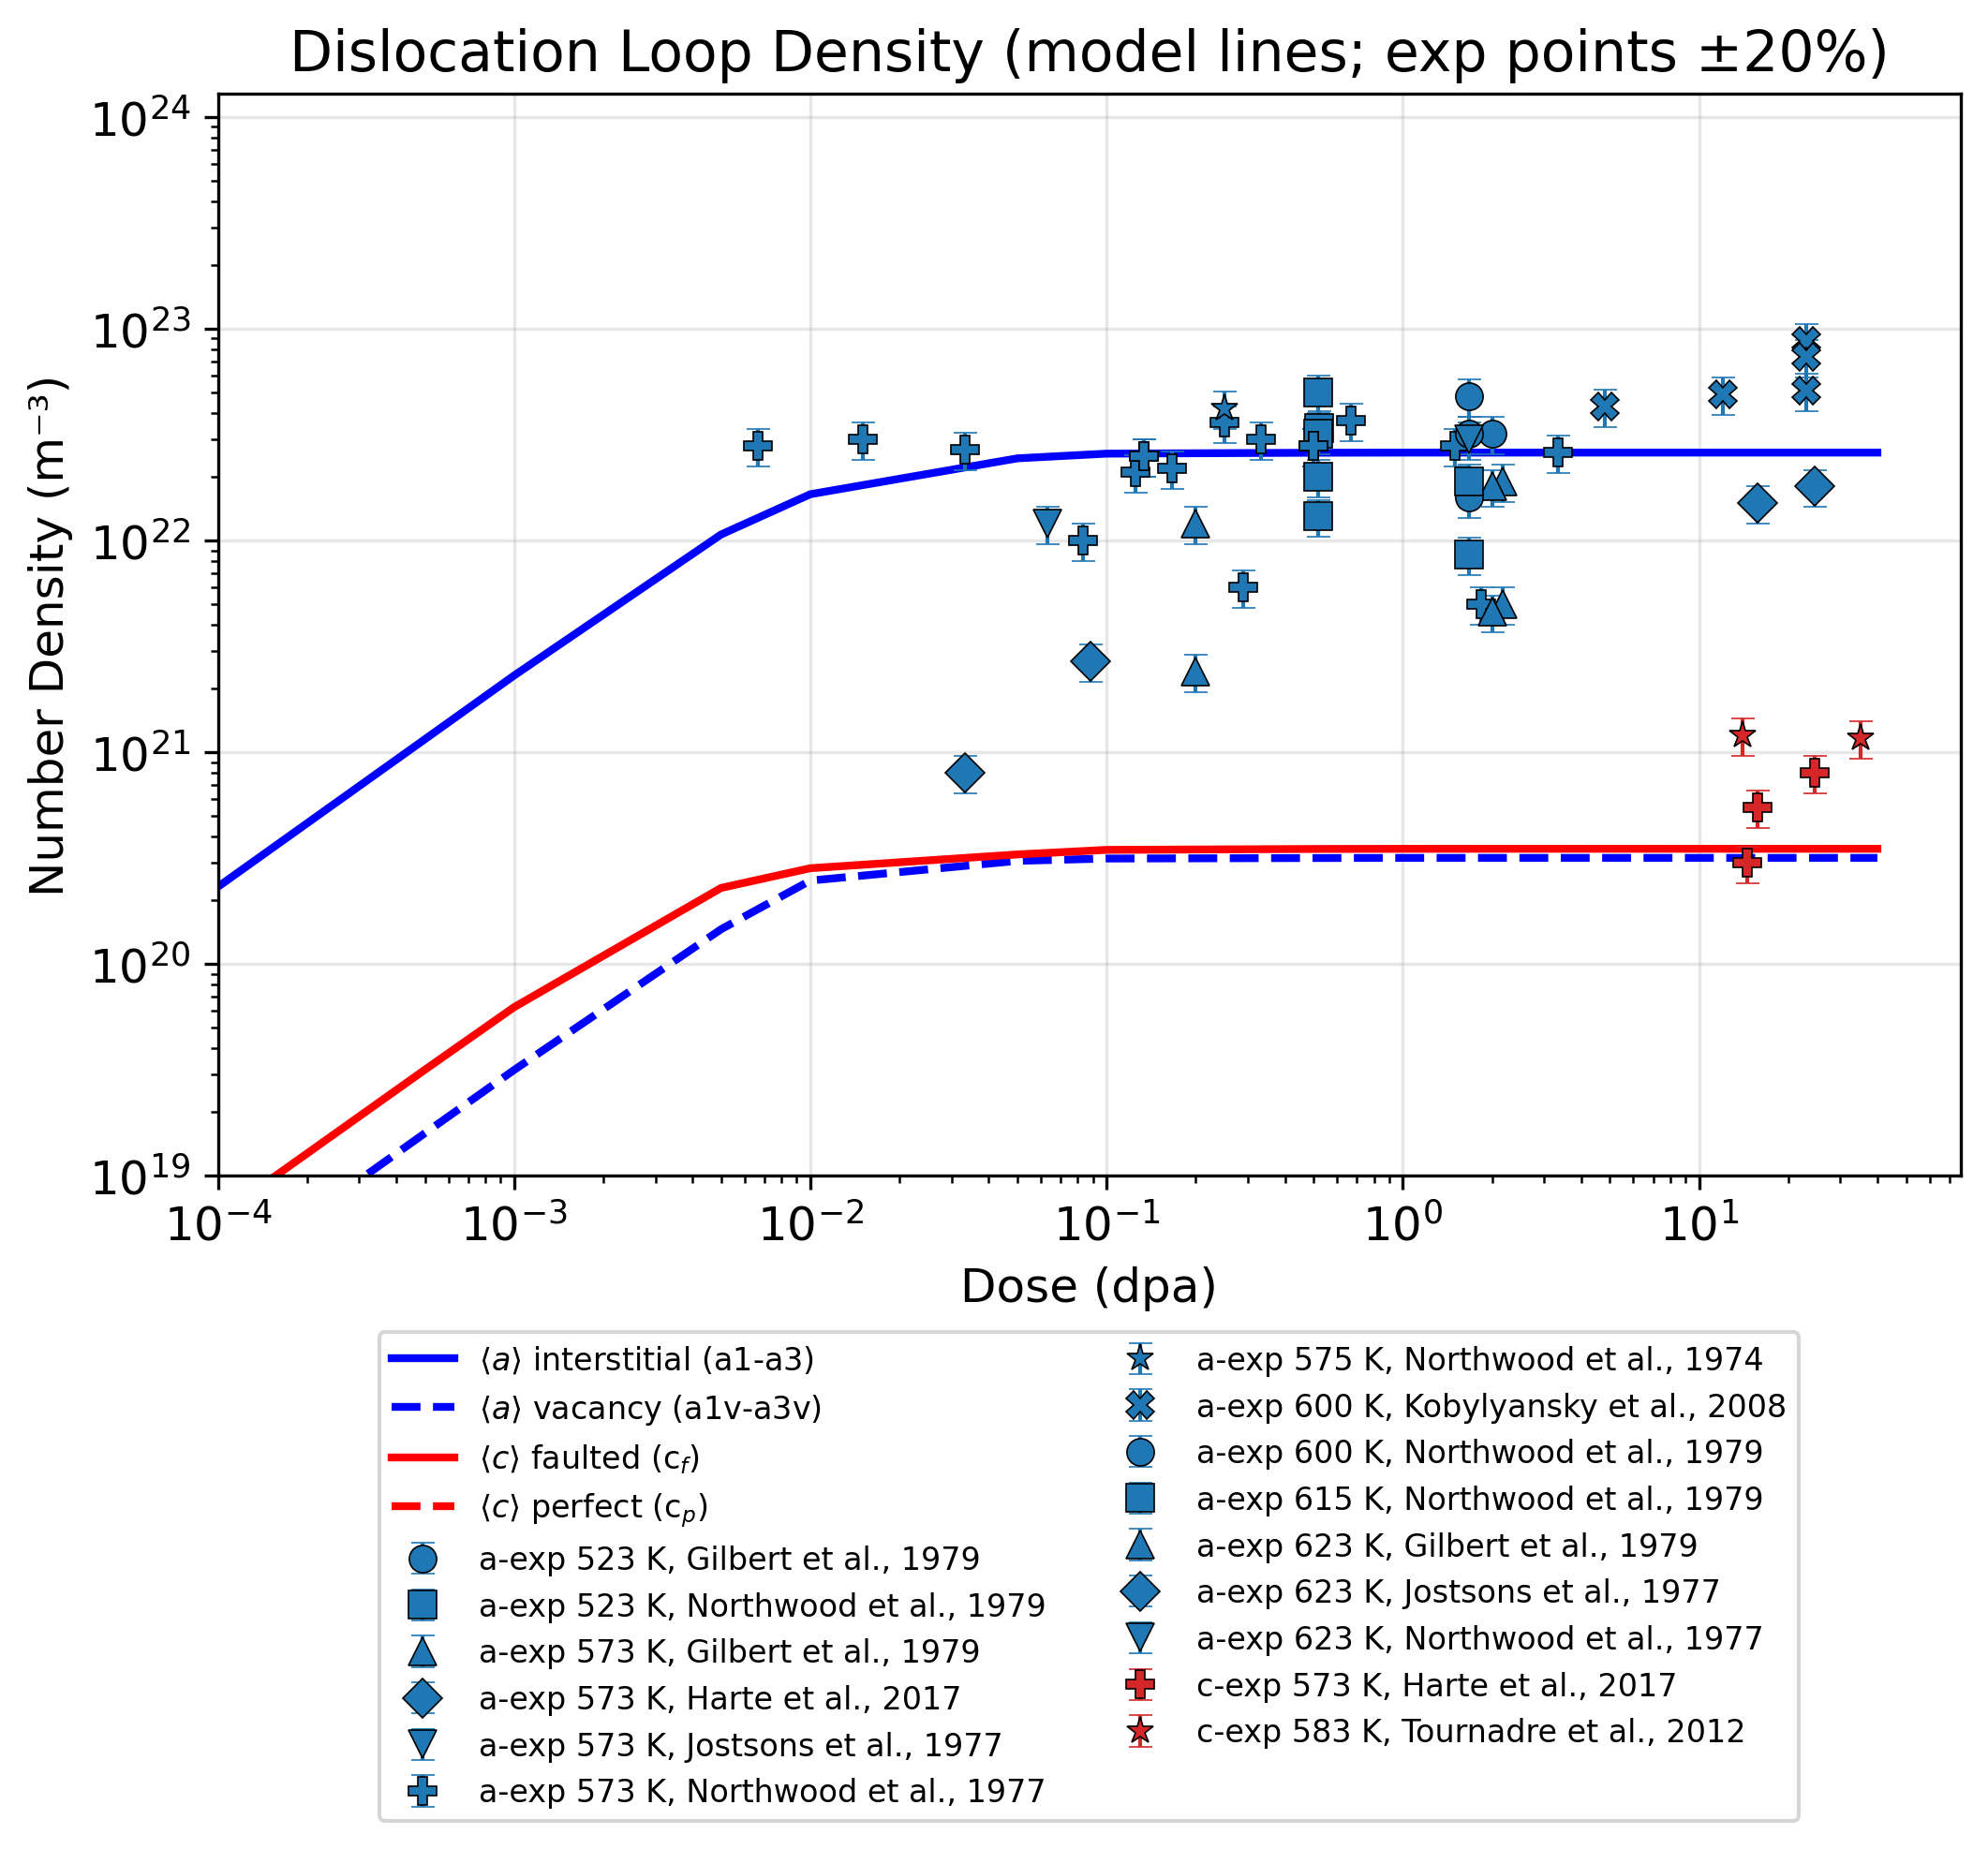
\includegraphics[width=\textwidth]{figures/loop_density.png}
\end{minipage}\hfill
\begin{minipage}{0.49\textwidth}\centering
  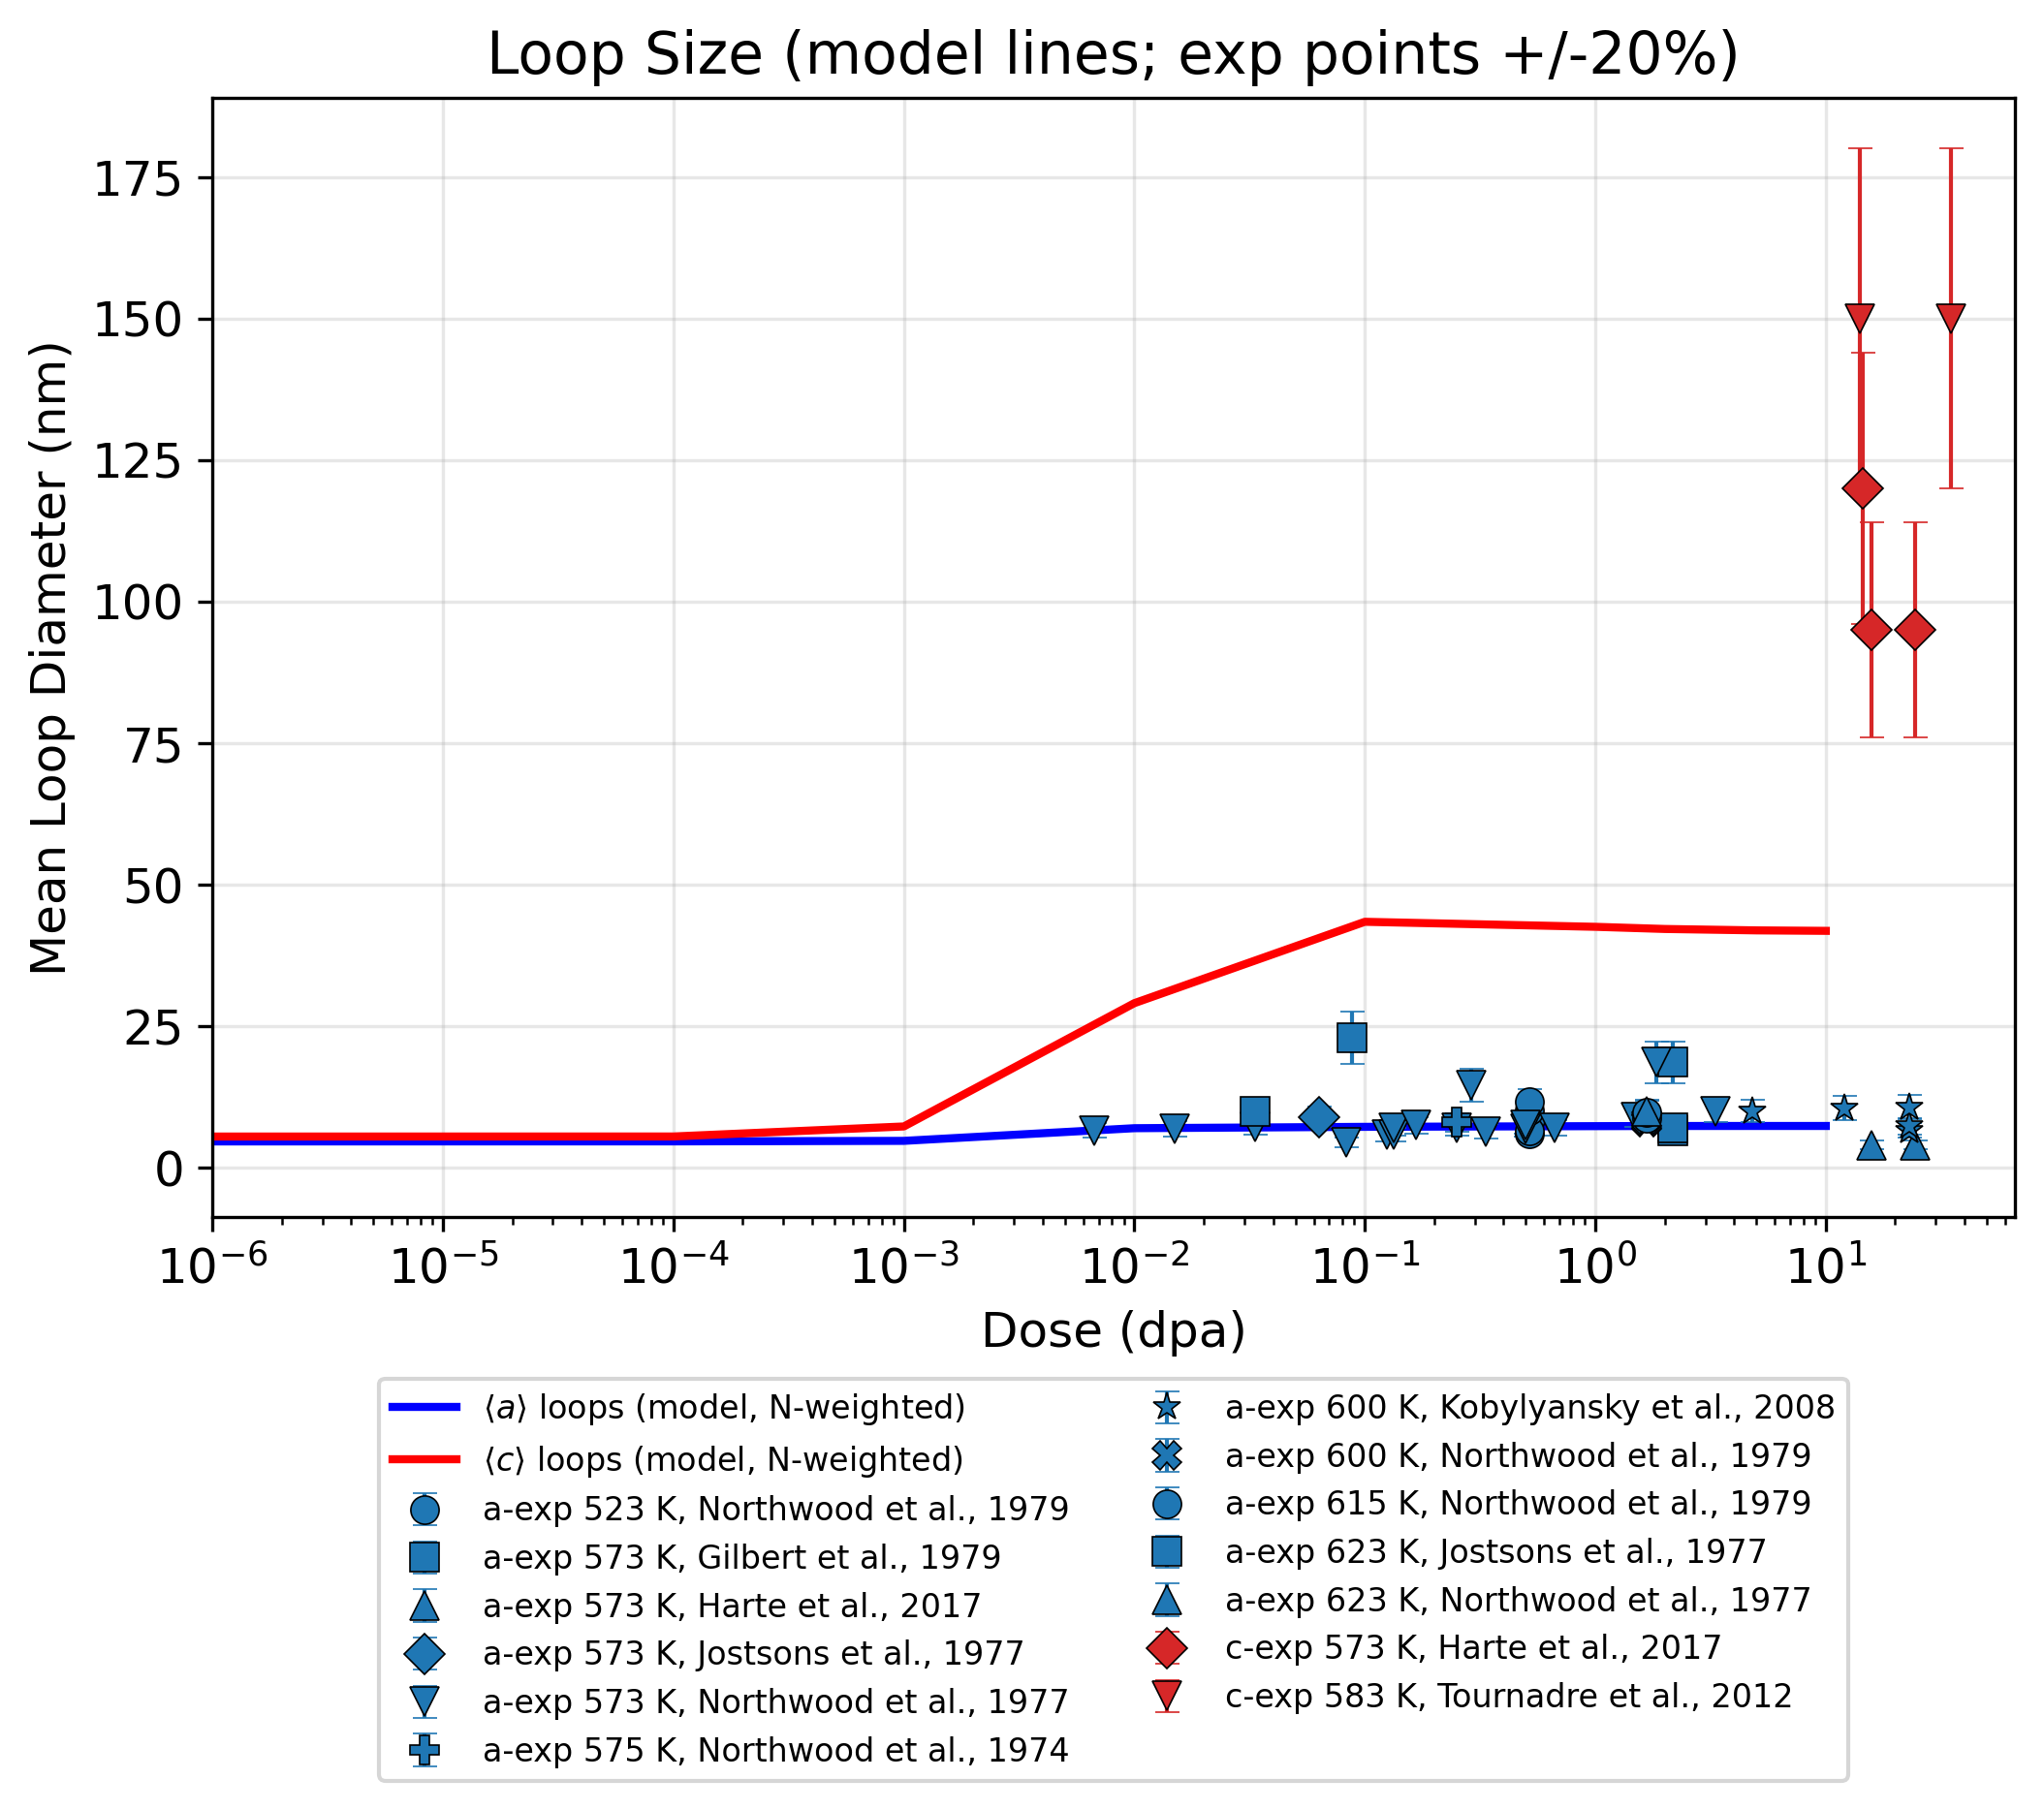
\includegraphics[width=\textwidth]{figures/loop_sizes_vs_exp.png}
\end{minipage}
\caption{Volume-averaged loop density against dose (left) and mean size against
the experimental measurements (right).}
\label{fig:volavg}
\end{figure}

\textbf{Which average is quoted is not a presentational choice.} On a Dirichlet
domain the boundary shell is a sink for mobile defects and --- without the
channel of \cref{sec:gb-loops} --- not a sink for loops, so it accumulates a
loop population that is numerous, tiny, and entirely unphysical as a description
of the material. At 10\,dpa:

\begin{center}
\begin{tabular}{@{}llrrrr@{}}
\toprule
& Region & $N_a$ (m$^{-3}$) & $d_a$ (nm) & $N_c$ (m$^{-3}$) & $d_c$ (nm) \\
\midrule
\multirow{2}{*}{loop channel off}
 & domain   & $1.32\times10^{24}$ & 5.01 & $1.41\times10^{24}$ & 5.74 \\
 & interior & $6.06\times10^{21}$ & 5.93 & $1.62\times10^{21}$ & 70.16 \\
\midrule
\multirow{2}{*}{loop channel on}
 & domain   & $4.61\times10^{21}$ & 7.41 & $6.74\times10^{21}$ & 37.07 \\
 & interior & $2.90\times10^{21}$ & 9.16 & $7.64\times10^{21}$ & 50.62 \\
\bottomrule
\end{tabular}
\end{center}

Without the channel the domain and interior means differ by a factor of $217$ in
$N_a$ and $873$ in $N_c$, and the domain-mean diameter \emph{falls} to 5.7\,nm
while the interior mean grows to 70\,nm --- the domain average is measuring the
boundary shell and nothing else. \textbf{With the channel the two agree to
within a factor of 1.6}, and a domain average becomes a statement about the
material. That is the strongest single argument for carrying the channel: it
removes an artifact that otherwise makes the most natural summary statistic
meaningless.

\paragraph{Against experiment, and the discrepancy.} At $573\,$K and 24.5\,dpa
the measurements give $N_c=8.0\times10^{20}\,\mathrm{m^{-3}}$ and
$d_c=95\,$nm. The interior of this calculation at 10\,dpa gives
$N_c/N^{\exp}=9.5$ and $d_c/d^{\exp}=0.53$: \textbf{too many loops, and too
small}. The companion without the loop channel gives $2.0$ and $0.74$ --- closer
on both, which is expected and is not an argument against the channel: the
parameters of \cref{tab:fitted} were fitted in a $0$-D that has no boundary at
all (\cref{sec:bias-caveat}), so the channel is an unmodeled loss acting on a
population calibrated without it. A refit with the channel active is required
before either number is quoted as a prediction.

The direction of the discrepancy is the informative part, and it is the same one
the calibration reported. The model produces \emph{more, smaller} \cloop{} loops
than are observed, and the two errors are linked: the number balance pins the
total content while the growth balance pins the size, so density is their
quotient and a model that removes loops faster than it grows them necessarily
has survivors that are too young. What the data want is \emph{fewer and larger},
and no channel exercised here achieves both. \Cref{sec:conclusions} states what
this implies.

\subsection{Continuum-to-discrete conversion}
\label{sec:results-discrete}

The conversion of \cref{sec:transfer} was applied to the fields at four doses.
The number of loops is not a parameter of the conversion: it is
$\sum_j n_j V_j$, the number the field says is present.

\begin{center}
\begin{tabular}{@{}lrrrr@{}}
\toprule
Family & $10^{-4}$\,dpa & $10^{-2}$\,dpa & 1\,dpa & 10\,dpa \\
\midrule
$c_f$ (basal, vacancy)          & 9 & 858 & 1031 & 1073 \\
$a_1$ (prismatic, interstitial) & 2 & 132 &   67 &   73 \\
$a_1^{v}$ (prismatic, vacancy)  & 2 &  87 &   56 &   61 \\
\bottomrule
\end{tabular}
\end{center}

\Cref{fig:discrete} shows the basal population at those four doses, drawn at
true radius and true position, over the continuum content field it was drawn
from. The two representations agree loop for loop: the figure is built from the
same draw the conversion exports, so a reader comparing this figure with the
exported loop table is comparing one object with itself.

\begin{figure}[htbp]
\centering
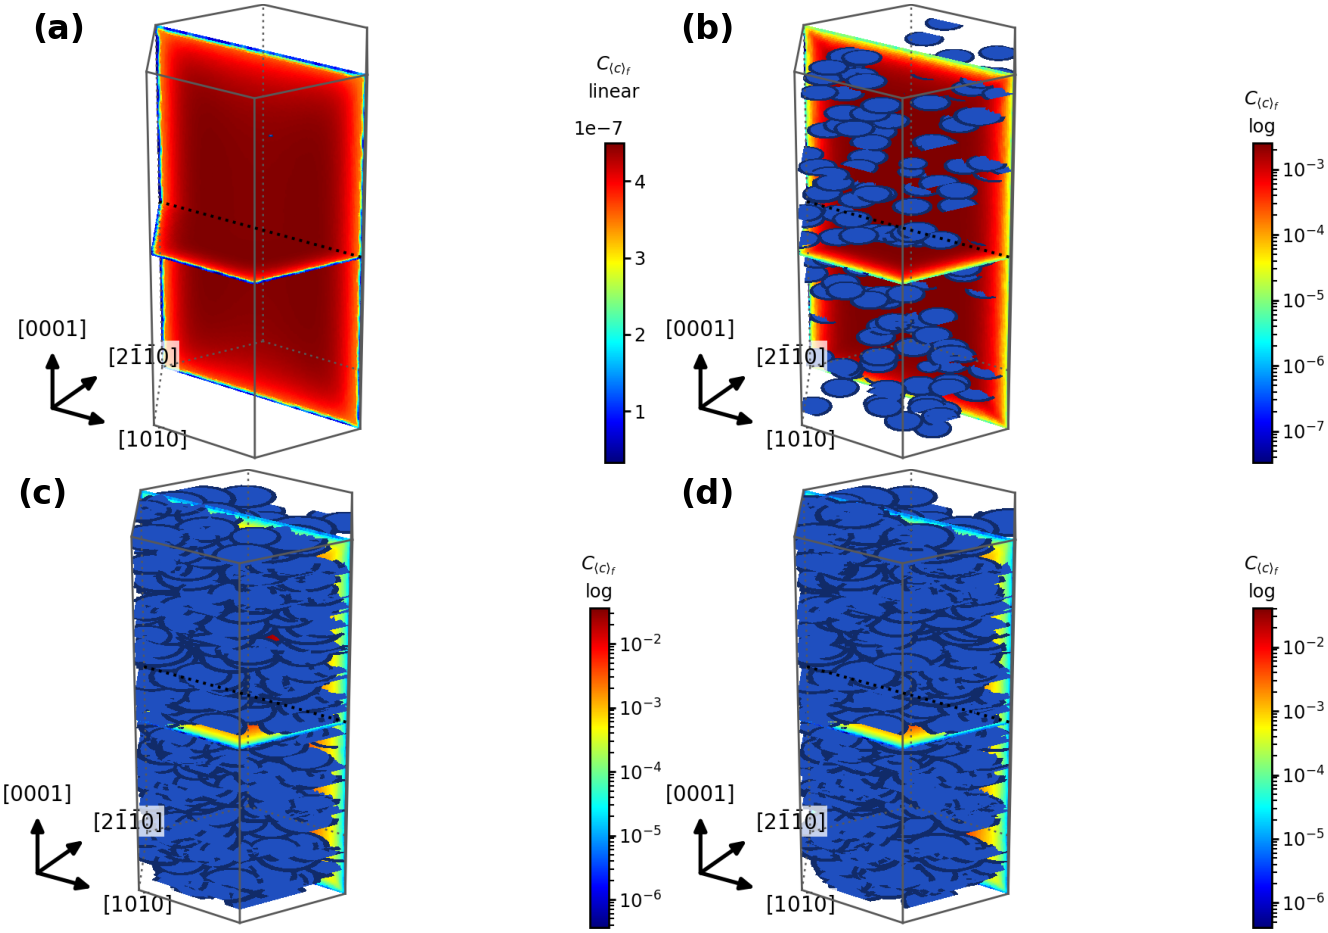
\includegraphics[width=\textwidth]{figures/loops_c_4dose.png}
\caption{The discrete basal \cloop{} population at (a) $10^{-4}$, (b) $10^{-2}$,
(c) 1 and (d) 10\,dpa, drawn at true radius over the continuum content field.
Counts are 9, 858, 1031 and 1073. The loops are clipped at the crystal surface;
see the text.}
\label{fig:discrete}
\end{figure}

\begin{figure}[htbp]
\centering
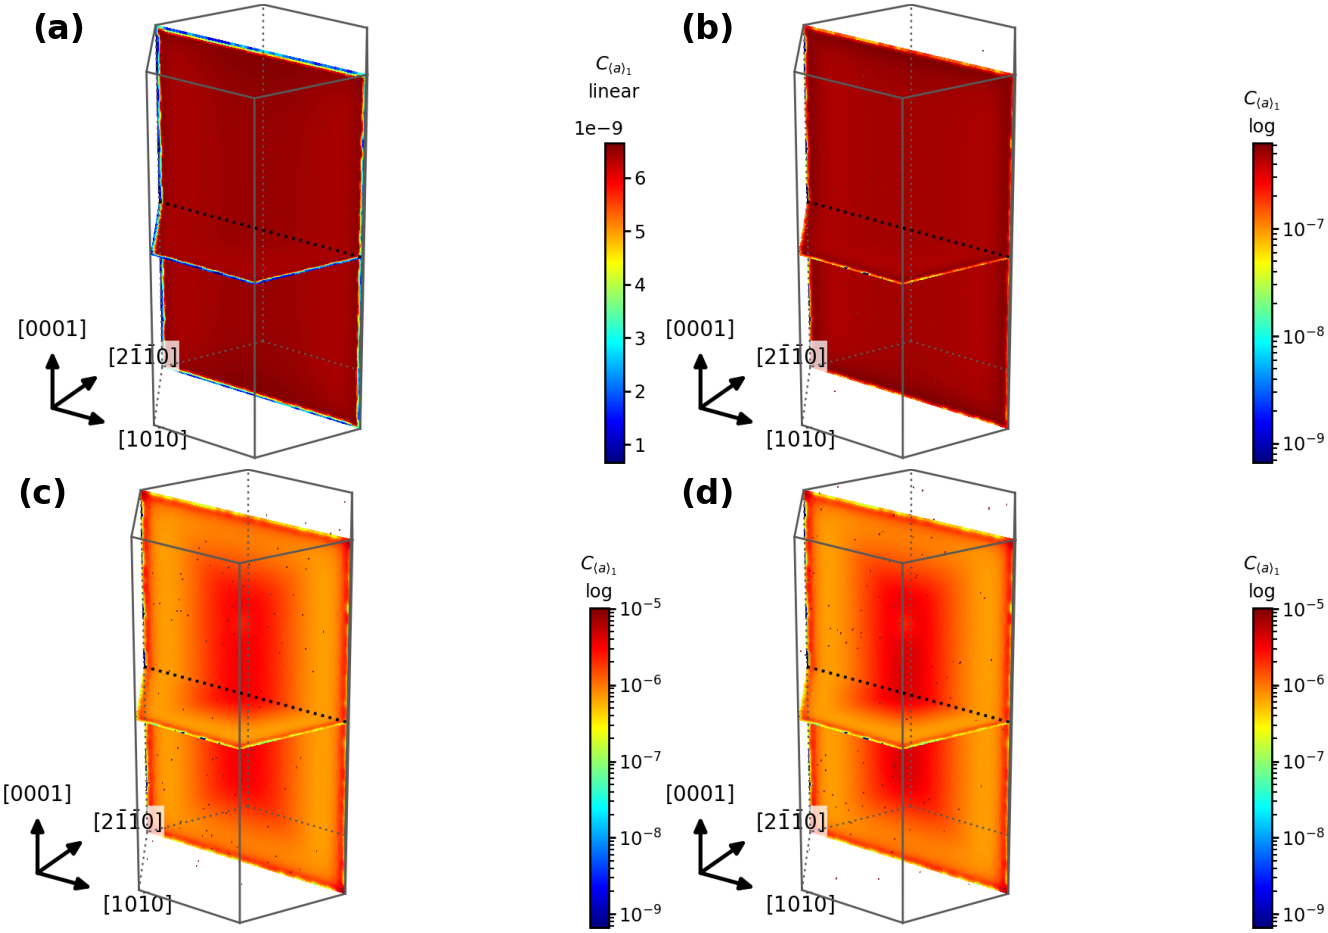
\includegraphics[width=\textwidth]{figures/loops_a1_4dose.png}
\caption{The discrete prismatic \aloop{}$_1$ population at the same four doses,
(a) $10^{-4}$, (b) $10^{-2}$, (c) 1 and (d) 10\,dpa, drawn at true radius.
Counts are 2, 132, 67 and 73. At true scale these loops are $6$--$7$\,nm across
in a \SI{500}{\nano\meter} crystal and are correspondingly sparse; the same
population drawn with exaggerated radii is legible but is not a population.}
\label{fig:discrete-a}
\end{figure}

Three observations.

\textbf{The count is not monotone, and it should not be.} Between $10^{-2}$ and
1\,dpa the prismatic count \emph{halves}, from 132 to 67, while the stored
content rises. That is coalescence: loops merge, so fewer, larger loops hold more
content. A conversion that preserved number rather than content would have hidden
this.

\textbf{A quarter of the basal loops do not fit.} At 10\,dpa, 287 of 1073
\cloop{} loops (26.7\%) are centered within their own radius of a face and
overhang it, by up to 40\,nm; the corresponding prismatic figure is 8.2\%. The
drawn population is clipped at the surface, but the clip is a drawing convention
and the exported loops are whole. This is the same geometric refusal that
\cref{sec:transfer} describes, and it means the basal handoff on a 500\,nm grain
is only partially feasible above $\sim0.1\,$dpa: a discrete-dislocation solver
would decline those loops, and their defects would have to remain in the
continuum. \emph{The correction to the \cloop{} Burgers vector that made the two
representations agree made this worse}, not better, because it raised the basal
radius by $\sqrt2$ and a larger loop is harder to fit.

\textbf{The conversion is where the mean field is checked against itself.} At
$10^{-4}\,$dpa the population is 9 basal and 2 prismatic loops in
$1.3\times10^{8}\,\mathrm{nm^{3}}$ --- a population so dilute that a continuum
density describing it is a statement about an ensemble and not about this
crystal. At 10\,dpa the basal loops are 50\,nm across with a mean spacing of
about 50\,nm, which is the opposite regime, and it is the one in which the
Avrami kernels of \cref{eq:avrami} are working hardest and are least defensible.
The conversion spans both, and the ledger of \cref{eq:ledger} closes on stored
defects to machine precision and on loop number to the integer draw at every one
of the four doses.
